%% ---------------------------------------------------------------
%% $URL: https://repository.cs.ru.is/svn/thesis-template/trunk/ruthesis/latex/DEGREE-NAME-YEAR.tex $
%% $Id: DEGREE-NAME-YEAR.tex 350 2018-03-07 22:41:33Z foley $
%% This is a template LaTeX file for dissertations, theses, or reports at Reykjavík University
%% 
%% Comments and questions can be sent to the RU LaTeX group (latex AT list.ru.is) 
%% ---------------------------------------------------------------

%% METHOD:
%% 0) Read ruthesis/thesis-instructions.pdf
%%    If it is missing, goto https://repository.cs.ru.is/svn/thesis-template/trunk/ruthesis/thesis-instructions.pdf
%% 0.2) Subscribe to the announcements email list at
%%    https://list.ru.is/mailman/listinfo/latex-announcements
%% 1 LaTeX instructions.tex or goto http://afs.rnd.ru.is/project/thesis-template/trunk/ruthesis/latex/instructions.pdf
%% 2) Copy the template files (or unzip) to your working area
%% 3) Rename this file (if needed) with your information e.g. MSC-FOLEY-2007.tex
%% 4) Modify this file to fit your needs (please follow all comments below in the text)
%% 5) For making bibliographies, run "biber".  You can also change
%%    this back to "bibtex".  See below in "Bibliography options".

%%%%%%% CHOOSE ONE OF THESE %%%%%%%%%%%%%%%
%% projectreport: Project report (CS)
%% bachelors: Bachelor of Science thesis
%% masters: Master of Science thesis
%% doctorate: Doctor of Philosophy dissertation
%
%%%%%%% CHOOSE ONE OF THESE %%%%%%
%% 
%% draft: speed up processing by skipping graphics and adding useful
%%     information for editing.  Also sets spacing to double so that it is easier to
%%     write editing marks on paper copy.
%% proof:  proofreading version (final formatting with warnings)
%% final: generate document for submission, removing FIXMEs, and
%%     other markup.  Throw error if any fatal FIXMEs still in document.
%%
%%%%%%% CHOOSE ONE OF THESE IF APPLICABLE %%%%%%
%%
%% deptsse: School of Science and Engineering
%% deptscs: School of Computer Science
%%
%%%%%%%% CHOOSE ANY COMBINATION OF THESE %%%%%%%%%%%%
%%
%% forcegraphics: force graphics, etc. to be included, even in draft mode
%% debug:  writes more messages to the log file, adds debugging output 
%%     and sizing boxes
%% icelandic: thesis is in Icelandic
%% oldstyle:  use the PhD headers and footers from the old CS template
%% online: for online versions (skip blank pages)
\documentclass[table,xcdraw,online,masters,deptsse,forcegraphics,draft]{ruthesis}

%%%%%%%%%%%%%%%%%%%% TeXStudio Magic Comments %%%%%%%%%%%%%%%%%%%%%
%% These comments that start with "!TeX" modify the way TeXStudio works
%% For details see http://texstudio.sourceforge.net/manual/current/usermanual_en.html   Section 4.10
%%
%% What encoding is the file in?
% !TeX encoding = UTF-8
%% What language should it be spellchecked?
% !TeX spellcheck = en_US
%% What program should I compile this document with?
% !TeX program = xelatex

%%%%%%%%%%%%%%%%%%%% Bibliography options %%%%%%%%%%%%%%%%%%%%%
%% We suggest switching from bibtex to biblatex/biber because it is better able
%% to deal with Icelandic characters and other bibliography issues
%% As long as you use biblatex instead of bibtex by itself, it will at least
%%  generate a document without errors.
%% !!!If you are using TeXStudio, don't forget to update the bibliography setting!!!
\usepackage[backend=biber,bibencoding=utf8,style=ieee]{biblatex}
%\DeclareLanguageMapping{american}{american-apa}  
% need to declare mapping for style=apa to alphabetize properly
% If you set backend=bibtex, it will use bibtex for processing (old way)
%    this can work with Icelandic characters, but you may get weird results.
%    bibtex does not know how to sort Þ and ð
% if you set backend=biber, you can use UTF8 characters such as Þ and
%     ð  but you will have to remember to switch from using bibtex to 
%     biber in your client
% If you use JabRef, make sure the file is encoded in UTF-8 which is
%    not the default.

%% This tells TeXStudio to use biber
% !TeX TXS-program:bibliography = txs:///biber
%% This also sets the bibliography program for TeXShop and TeXWorks
% !BIB program = biber

% Where is your reference library?
\addbibresource{references.bib}

%%%%%%%%%%%%%%%%%%% CUSTOMIZATIONS %%%%%%%%%%%%%%%%%%%%%%%%%%%%%
%% It is not recommended that you customize this file nor
%% ruthesis.cls.  Just fill in the necessary fields.  You should put
%% your macros and packages into a separate file so that it is easier
%% to use updates to the template.  The custom.sty file was created
%% for this reason.  We load this much later so that it can overrite
%% any existing settings
\IfFileExists{custom.sty}{\usepackage{custom}}{}

%%%% My user packages-Toma%%%%%%
\usepackage{multirow}
%\usepackage[table,xcdraw]{xcolor} %% this was added to the \documentclass[..here..]
% \usepackage{refcheck}
% \usepackage{showlabels}% !!!remove this in final version!!!


%%%%%%%%%%%%%%% INFORMATION %%%%%%%%%%%%%%%%%%5
%% University information must be multilingual to deal with the
%%  required cover pages and abstract on thesis
%% NOTE: This may not be required for other reports!!!

%% Babel Icelandic macros are setup  on RedHat at
%% /usr/share/texlive/texmf-dist/tex/generic/babel/icelandic.sty
%% /usr/share/texlive/texmf-dist/tex/generic/babel-icelandic/icelandic.ldf


%% Multilingual macros
%\newML{macroname}{englishword}{icelandicword}
%  creates \macronameML
%    \MLmacroname[english] - returns the english word
%    \MLmacroname[icelandic] - returns the icelandic word
%    \MLmacroname  - uses the current language setting
% Some useful ones have already been defined, but can be redefined
%% Predefined: \MLIceland \MLReykjavikUniversity \MLUniversityIceland

%% What institute?  Default is RU.
%\setInstitution{\MLReykjavikUniversity}
% \newML{InstitutionAddress}{Menntavegur 1\\101 Reykjavík, Iceland}
% {Menntavegi 1\\101 Reykjavík, Ísland}
% \setInstitutionAddress{\MLInstitutionAddress}
% \newML{Tel}{Tel.}{Sími}
% \setInstitutionPhone{\MLTel{} +354 599 6200\\
% Fax +354 599 6201}
% \setInstitutionURL{www.ru.is}


%% ONLY SET DEPARTMENT IF YOU HAVE NOT USED THE deptsse or deptscs OPTION!
%% Department and degree program
%\newML{ND}{New Department}{Nytt deild}
%\setSchool{\MLND}

%% Set your program of study
\newML{program}{Mechanical Engineering}{vélaverkfræði}
\program{\MLprogram}

%% Degree long name.  If not already defined, you can create a macro
%\newML{DEGREE}{English Degree Name}{Icelandic Degree Name}
%% Default is set based upon doctorate vs masters option
%% Predefined: \MLMSc \MLPhd
%\setDegreelong{\MLMSc}

%% Degree abb, change if default is not right
%% Default is set based upon doctorate vs masters option
%\degreeabbrv{Sc.D.} 

%\setFrontLogo{reyst-logo}
%% Use this if you need a different front logo on the first page
%% e.g. reyst-logo

%% Date in english and icelandic
%% NOTE: THIS IS THE DATE OF THE SUPERVISOR'S SIGNATURE!!!!!!
%% Predefined: \MLjan, \MLfeb, \MLmar, ... \MLdec
%\whensigned{day}{month}{year} %day is only used on some formats, but you must put something.
\whensigned{10}{\MLjan}{2019}

%% Title in English and Icelandic
%% You need to put both a normal case and ALL CAPS version into the macros.
%%
%% Note that title length is limited to what can fit in three lines in the inside page
\newML{Title}{Wake Vortex Separation Re-categorization Requirements (RECAT) for Keflavik Airport}{Titll verkefnis}
%\newML{Title}{Working Title}
\newML{TITLE}{WAKE VORTEX SEPARATION RE-CATEGORIZATION REQUIREMENTS (RECAT) FOR KEFLAVIK AIRPORT}{TITLL VERKEFNIS}
%% If you have the title in just one language, put it into \setTitle{} directly e.g.
%%  \setTitle{Working Title}
%%
\setTitle{\MLTitle}{\MLTITLE}
%% ***** Special Titles ******
%% If the title must be formatted specifically for the cover page or internal pages
%% (typically via line-breaks using the \newline command) then the following commands must be used 
%%
%\setTitleCover{\MLTITLE}
%% These two for the internal cover pages, usually not needed
%\newML{TitleInternal}{Internal Title}{Icelandic Internal Title}
%\setTitleInternal{\MLTitleInternal}

%% Author name (should be the same in any language, if not use \newML)
%% If you are writing a Project report with multiple authors, separate them with \\:
%% To keep the names typeset together, you want to use non-breaking spaces: ~
%% TODO: fix formatting for TVD BSc multi-author (x4) --foley
%\author{Firstname1~Lastname1\\Firstname2~Lastname2}
\author{Toma~Emilov~Tomov}

%% If the name must be formatted specifically for the signature page
%% (typically via line-breaks) then the following command must be used 
%\setAuthorSignature{Student\\Name}
%% This macro adjusts the author name in the headers of the oldstyle formatting
%\setAuthorHeader{StudentLast}

%%% TODO:  Move the bachelor's form separately -- it confuses people. --foley
%%%%%%%%%%%%%%%%%%%%%%%%%% Project Report or Bachelor's Only!!! %%%%%%%%%%%%%%%%%%%%%%%%%%%%%%%%%%%%%%%%%%%
\setCourse{VT LOK 1012}

%%%%%%%%%%%%%%%%%%%%%%%%%% Bachelors Only!!! %%%%%%%%%%%%%%%%%%%%%%%%%%%%%%%%%%%%%%%%%%%
% \setID{010105--9999}%kennitala
% \setSemester{2016--1}
% \setShortSignedDate{1.1.2016}

% \setOrganization{Marel ehf.\\Austurhrauni 9\\210 Garðabær}
% \setSubProgram{Tæknifræði}

% %% If the thesis is confidential, uncomment this with the date it can be released
% %\setClosedDistribution{10.1.2016}%

% %% Put your keywords here in English, then Icelandic.  Separate them with commas.
% \newML{keywords}{Keyword1, Keyword2, Keyword3}{Lykliorð1, Lykliorð2, Lykliorð3}
% \setKeywords{\MLkeywords}

%%%%%%%%%%%%%%%%%%%%%%%%%%% Masters Only!! %%%%%%%%%%%%%%%%%%%%%%%%%%%%%%%%%%%%%%%%%%%%
%% How many credits (ECTS) on Master's degree
%% Usually 30 or 60
\ects{30}

%%%%%%%%%%%%%%%%%%%%%%%%%%% Doctorate Only!! %%%%%%%%%%%%%%%%%%%%%%%%%%%%%%%%%%%%%%%%%%
%% Some Computer Science Thesis have an ISSN number.
%% Most other documents do not.
%\bookidnumber{ISSN: 1670-8539} 
%% ID numbers are optional, but nice for sorting in libraries

%% International Standard Book Number (ISBN)
%% This is what most people should use if the thesis is being published.

%% International Standard Serial Number (ISSN)
%% This is usually only for a PhD dissertation as part of a series when published
%%   Computer Science: 1670-8539 

%% Additional degrees?  (optional, usually not needed)
%\adddegree{(list of degrees in appendix)}{(sjá lista yfir prófgraður í viðauka)}
%%%%%%%%%%%%%%%%%%%%%%%%%%%%%%%%%%%%%%%%%%%%%%%%%%%%%%%%%%%%%%%%%%%%%%%%%%%%%%%%%%%%%%%%


%% List the entire committee.  Each member has a name (degree should be omitted, unless it is not PhD),
%% Supervisor(s) must appear first
%% On a Bachelors, there is usually only one supervisor and one examiner.

%% Format for each entry:
%%  \personinfo{Name}{Role}{Job Title}{Company/institution}{Country}
%% Predefined macros: \MLSupervisor \MLSupervisors \MLExaminer \MLExaminers

%% Change these to singular/plural as needed.
%% Just uncomment and change the plurality of the macro.
\setSupervisorHeading{\MLSupervisors}
\setExaminerHeading{\MLExaminer}

%% Predefined macros:
%% \MLSeniorProfessor \MLProfessor \MLAssociateProfessor \MLAdjunctProfessor \MLEmeritusProfessor \Iceland
%% \MLReykjavikUniversity \MLUniversityIceland

%% Bachelors: primary advisor (Umsjónarkennari), ONLY ONE!
%% All others: As many as you want
\supervisors{
  \personinfo{Þorgeir~Pálson}{\MLSupervisor}{\MLProfessor~Emeritus}{\MLReykjavikUniversity}{\MLIceland}
  \personinfo{Ármann~Gylfason}{Co-advisor}{\MLAssociateProfessor}
  {\MLReykjavikUniversity}{\MLIceland}
%  \personinfo{Helper A. Bunch}{Co-advisor}{\MLAssistantProfessor}{\MLUniversityIceland}{\MLIceland}
%  \personinfo{Ian M. Great}{Co-advisor}{\MLProfessor}{Hochschule Düsseldorf}{Germany}
}

%% Bachelors: secondary advisor (Leiðbeinandi), ONLY ONE
%% All others: As many as you want
\examiners{
  \personinfo{Tough E. Questions}{\MLExaminer}{Associate Professor}{Massachusetts Institute of Technology}{USA}

}

%% An abstract is required to be in both Icelandic and English for most degrees.
%% It is considered good form to limit the abstract to a single paragraph in each language,
%%   at 300 words.  Refer to your degree's instructions.
%% Note: Icelandic quotation marks cannot be typeset using "` and "'.  You should use \enquote{}
%% this is probably due to interactions with the MultiLingual macros.
%% TODO: turn this into more sensible macros to avoid confusion --foley
\newML{AbstractText}{\lipsum[1]}  
% ipsum generaes text text
{\lipsum[1]} % Icelandic abstract goes here
\setAbstract{\MLAbstractText}


%%%%%%%%%%%%%%INDEX SETUP %%%%%%%%%%%%%%%%%%%%%%%%%%%%%%%%%%%%%%%%%%%%%%%%%%%%
%% Indexes, and other auto-generated material
%% The Memoir package (which we use) automatically generates the index
%% See section 17.2 on page 302 of the guide
%% http://texdoc.net/texmf-dist/doc/latex/memoir/memman.pdf
%% This means you have to run "makeindex DEGREE-NAME-YEAR"
%% !!!Do not load any of the index packages, they cause problems with Memoir!!!
%% !!!You have been warned!!!
%% Note that memoir changes the [] options to only be for filenames, not other options!
\makeindex{}
\indexintoc{}

%% For abbreviations, you may want to try
%% Watch out though, each new index writes another external file and 
%% latex can only write a limited number of them
%%\usepackage[intoc]{nomencl} % intoc: In Table of Contents
%% remember to run:
%% makeindex filename.nlo  -s nomencl.ist -o filename.nls

\finalifforcegraphics{hyperref} %hyperlinks even in draft mode
\usepackage[hidelinks]{hyperref} 
%% !!!Must be the last package loaded except otherwise mentioned!!!!
%% \usepackage{hypcap}  %% puts link at top of figure, must be after hyperref

%%%%%%%%%%%%%%%%%%%%%%%%%%%%%%%%%%%%%%%%%%%%%%%%%%%%%%%%%%%%%%%%%%%%%%%%%%
%%%%%%%%%%%%%%%%%%%%%%% DOCUMENT START %%%%%%%%%%%%%%%%%%%%%%%%%%%%%%%%%%%
\begin{document}
%% Some elements have different names on the RU Masters rules
%% They will be annotated with RUM: "name"
\frontmatter{} % setup formatting at beginning

%\frontcover{}%%If you want to see what it looks like with the printed cover
%% TODO:  link to fill-in PDF file on RU website

\frontrequiredpages{}%% the various signaturepages and abstract
%%% WARNING:  if you get an error on the previous line, it is probably because
%%% you put a bad macro or something strange in a title, author, or abstract.

\ifdraft{\coverchapter{Important!!!  Read the Instructions!!!} If you
  have not already done so, \LaTeX{} the \path{instructions.tex} to
  learn how to setup your document and use some of the features.  You
  can see a (somewhat recent) rendered PDF of the instructions included in this folder at\path{instructions-publish.pdf}.
  There is also more information on working with \LaTeX{} at
  \url{http://afs.rnd.ru.is/project/htgaru/trunk/how-to-get-around-projects.pdf}.
  This includes common problems and fixes.

  This page will disappear in anything other than draft mode.}{}



%% Dedication is optional, comment out if it is absent
%% RUM: Not mentioned
% \begin{dedications}
%   I dedicate this to my two cats, Sid Vicious and Nina Hagen.
% \end{dedications}

\enableindents{}% turn on/off paragraph indents
% RUM: "Acknowledgements (optional)"
\coverchapter{Acknowledgements} 
% \begin{quotation}
% So long, and thanks for all the fish.
% \end{quotation}\sourceatright{Douglas Adams\cite{adams84fish}}
% \vspace{\baselineskip}

\draftnote{Acknowledgements are optional; comment this chapter out if they are absent
  Note that it is important to acknowledge any funding that helped in the work.}

The work on this thesis was supported by \the\year~Isavia funds.
Additionally the company provided a workplace and the means to obtain the necessary information from the company servers. Special appreciation goes to Hjalti Pálsson, Head of Research and Development Department and his team of professionals: Atli Norðmann Sigurðarson, Specialist, for valuable insight into the manner of retrieving and analysing the data, Víkingur Logi Ásgeirsson, Project Manager, for his beneficial assistance in managing the specifics of the Python code.

% \coverchapter{Preface}
% % RUM: "Preface (optional)"
% This dissertation is original work by the author, Firstname~Lastname.
% Portions of the introductory text are used with permission from
% Student et al.\cite{student2015awesome} of which I am an author.

  
% \draftnote{The preface is an optional element
%   explaining a little who performed what work.  See
%   \url{https://www.grad.ubc.ca/sites/default/files/materials/thesis_sample_prefaces.pdf}
%   for suggestions.
  
%   List of publications as part of the preface is
%   optional unless elements of the work have already been published.
%   It should be a comprehensive list of all publications in which
%   material in the thesis has appeared, preferably with references to
%   sections as appropriate.  This is also a good place to state
%   contribution of student and contribution of others to the work
%   represented in the thesis.}

%\coverchapter{Publications}
%% RUM: Not mentioned, this was found in the CS thesis template.  
%% Maybe more applicable to PhD dissertations?
%%% Probably a duplication from before Preface became standard.

\starttables{}% setup formatting
%% TOC, list of figures and list of tables are required
\tableofcontents{}\clearpage%%RUM: "Table of contents"
\listoffigures{}\clearpage%%RUM: "List of figures"
\listoftables{}\clearpage%%RUM: "List of tables"

%\coverchapter{List of drawings and enclosed material}
%RUM: "List of drawings and enclosed material, e.g. CD(as appropriate)"

\listoffixmes{}
% if using fixme package, lists what needs to be done

%% The list of abbreviations is an example of a special list
%% Other lists may be added, such as lists of algorithms, symbols, theorems, etc.
%% IN CS PhD, this is sometimes centered.
\coverchapter{List of Abbreviations}%%RUM: Not mentioned

\begin{tabular}{ll}
% MSc     &   Masters of Science\\
% PhD   &   Doctor of Philosophy\\
 ADS-B   &   Automatic Dependent Surveillance-Broadcast\\
 AROT    &   Arrival Runway Occupancy Time\\
 ATM     &   Air Traffic Management\\
 B-C     &   CAT-B leader - CAT-C follower RECAT pair\\
 B-D     &   CAT-B leader - CAT-D follower RECAT pair\\
 BIKF    &   Keflavík International Airport ICAO code name\\
 C-C     &   CAT-C leader - CAT-C follower RECAT pair\\
 C-D     &   CAT-C leader - CAT-D follower RECAT pair\\
 C-F     &   CAT-C leader - CAT-F follower RECAT pair\\
 D-C     &   CAT-D leader - CAT-C follower RECAT pair\\
 D-D     &   CAT-D leader - CAT-D follower RECAT pair\\
 D-F     &   CAT-D leader - CAT-F follower RECAT pair\\
 EASA    &   European Aviation Safety Agency\\
 FAA     &   Federal Aviation Administration\\
 H-H     &   Heavy leader - Heavy follower ICAO pair\\
 H-M     &   Heavy leader - Medium follower ICAO pair\\
 IATA    &   International Air Transport Association\\
 ICAO    &   International Civil Aviation Organisation\\
 IFR     &   Instrumental Flight Rules\\
 KEF     &   Keflavík International Airport IATA code name\\
 LTI     &   Landing Time Interval\\
 M-H     &   Medium leader - Heavy follower ICAO pair\\
 M-M     &   Medium leader - Medium follower ICAO pair\\
 MOPS    &   Minimum Operational Performance Standards\\
 MRS     &   Minimum Radar Separation\\
 MTOM    &   Maximum Take-off Mass\\
 MTOW    &   Maximum Take-off Weight\\
 NACp    &   Navigation Accuracy Code for position\\
 NIC     &   Navigation Integrity Code\\
 NM      &   Nautical mile\\
 NUC     &   Navigation Uncertainty Code\\
 PIC     &   Position Integrity Code\\
 RECAT-EU   &   European Wake Turbulence Categorisation and Separation Minima on Approach and Departure\\
 ROT     &   Runway Occupancy Time\\
 RWY     &   Runway\\
 SIL     &   Surveillance Integrity Level\\
 TWY     &   Taxiway\\
 VFR     &   Visual Flight Rules\\
 WTC     &   Wake Turbulence Category\\

\end{tabular}


% \coverchapter{List of Symbols}%%RUM: Not mentioned
% \begin{tabular}{lll}
% Symbol &Description &Value/Units\\
% $E$ &Energy &\si{\joule}\\
% $m$ &Mass &\si{gram}\\
% $c$ &Speed of Light &\SI{2.99E8}{\meter\per\second\square}\\
% \end{tabular}

%% This command prepares for the actual text, e.g. by 
%% calling \mainmatter{}
\starttext{}

%% ---------------------------------------------------------------
%% From this point on, it is standard Latex, except the very end.
%% This is a "report"-based template, so the top-level heading 
%% is \chapter{}

%% WARNING: Make sure that all of these files (and any new ones)
%% are UTF-8 otherwise you will get weird encoding errors.
% \part{The First Part} % Parts optional but useful in longer documents

%% The default division is IMRAD, you may want to divide differently
%% See the introduction for guidance.

\chapter{Introduction\label{cha:introduction}}
%% \ifdraft only shows the text in the first argument if you are in draft mode.
%% These directions will disappear in other modes.
% \ifdraft{State the objectives of the exercise. Ask yourself:
%   \underline{Why} did I design/create the item? What did I aim to
%   achieve? What is the problem I am trying to solve?  How is my
%   solution interesting or novel?}{}

Keflavík International Airport (IATA:KEF, ICAO:BIKF) is the major gateway to Iceland currently with two functioning runways. The runways operate in both directions and are designated as RWY-01 (South-North), RWY-19 (North-South) , RWY-10 (West-East) and RWY-28 (East-West). 
There has been a gradual increase of passengers travelling through Keflavík Airport in the recent years with over eight million passengers and 62,3 thousand air transport movements in 2017~\cite{isavia_facts_2017}. For 2018 the passenger numbers show a growth of 13.1\% on average (at the time of writing) from the previous year~\cite{isavia_pass_statistics_2018}. The increase in traffic at Keflavík Airport can encounter constrained capacity of the runways during peak traffic periods. 
A significant constraint of airport capacity is caused by separation regulations of aircraft due to wake-vortices. These are specified by rules established by the European Aviation Safety Agency (EASA) for each type of aircraft based primarily on the weight of the aircraft. The general flight safety requirements are established by the International Civil Aviation Organisation (ICAO) for maintaining safe distance between aircraft.\fxnote{Introduction needs more work, incomplete.}

\section{Background and Literature Review}
The research parameters for the literate review included but were not limited to the following concepts: runway occupancy time, runway capacity, wake vortex separation. The project addresses in particular the arrival runway occupancy and its seasonal fluctuations as well as the variations between the different runways at Keflavík International Airport.
%\ifdraft{Provide background about the subject matter (e.g. %How was morse code developed?  How is it used today?). 
%This is a place where there are usually many citations.
%It is suspicious when there is not.
%Include the purpose of the different equipment and your %design intent. 
%Include references to relevant scientific/technical work and %books.
%What other examples of similar designs exist?
%How is your approach distinctive?

%If you have specifications or related standards, these %mustscribed and cited also.  As an example, you might cite %the specific
%RoboSub competition website (and documents) if working on the %lighting system for an AUV

%%% Glossary is broken, do not use --foley
%% \gls{auv}\footnote{Autonomous Undersea Vehicle}.
%
%% Notice that there is now information on the AUV in the %Index %and Acronyms.
%% It isn't in the \gls{glossary} because we didn't put it %there.
%\index{AUV}
%}{}



\subsection{Current Understandings of Wake Vortex Behaviour}

The lift effect on wing is created by the differential pressure between the lower and the upper surface of the wing. At the wing tips the high pressure flow from the lower side leaks around the tip and to the upper side of the wing. Thus the streamlines over the wing are pushed inwards, while the streamlines under the wing are pushed outwards. When the two streams combine at the trailing edge of a lifting wing, the difference in span-wise velocity causes the air to roll up into a number of small stream-wise vortices distributed along the span of the wing that eventually mix together and combine into two main counter-rotating vortices aft of the wing as illustrated in Figure~\ref{fig:vortex_develop} ~\cite{houghton2012aerodynamics,magazine_aibus_safety, Breitsamter2011Feb, gerz_commercial_2002}. Between the vortices the induced flow is downwards (downwash) while outside the air moves upwards. Those vortices are also known as wake turbulence. 
The kinetic energy contained in the vortices is dependent on the weight and aerodynamics of the generating aircraft. The cross flow velocities in the core region of the trailing vortices can reach $360$ km/h and the vortices can stay effective up to hundred wing spans, which can result in wake vortices lasting for several minutes and up to $30$ km behind larger aircraft~\cite{Breitsamter2011Feb, gerz_commercial_2002}. 

\begin{figure}[ht]
    \centering
    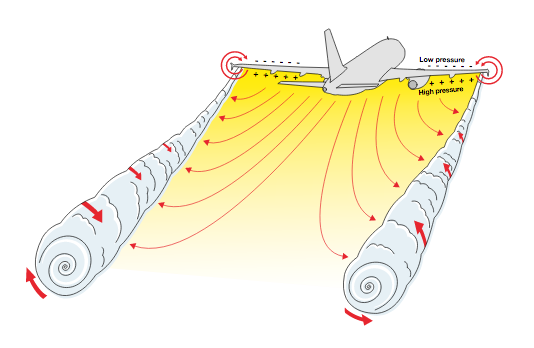
\includegraphics[width=0.8\textwidth]{graphics/WakeVortexPlane.png}
    \caption[Wake vortex roll-up process]{Wing vortex evolution and roll-up process. Two main vortices form behind the aircraft turning in opposite directions, clockwise behind the left wing (seen from behind) and anti-clockwise behind the right one~\cite[p. 043]{magazine_aibus_safety}} \label{fig:vortex_develop}
\end{figure}

\subsection{Ground Effect and Decay Process}

Near ground on approach the wake vortices tend to descend slowly to an altitude of about one half of the initial separation.
Upon reaching this point the descent will stop and then ascend slowly. This "re-bounce" effect is caused by the presence of the ground and carries with it the formation of a second pair of induced vortices outside and bellow the main vortex. 
In the presence of stable cross-wind conditions the decay of the downwind vortex is not identical to the upwind vortex and the descent rate may vary significantly \cite{Hallock2018Apr}. 
The trajectories of the vortex pair may be modified and the upwind vortex could stall over the runway while the downwind vortex ascends and decays faster (Figure~\ref{fig:vortex_ground_effect}).
Measurements have shown that the lateral/sideways motion of a vortex in an airport environment could range between $229$~m and $518$~m and in some cases even $762$~m, which is the basis for the "2500-foot"  rule separation in parallel runways configuration~\cite{Hallock2018Apr, hallock2004summary, hallock2003wake}. The vertical descent rate of vortices for medium commercial aircraft in stable atmosphere  is shown to be around $1.5-2.5$~m/s for the first $30$~s after which the descent slows and eventually approaches zero at $152-274$ m below the flight path, and for heavier aircraft decaying vortices have been observed at $305$~m and below of the flight path~\cite{lissaman1973aircraft, Hallock2018Apr}. 
Aerodynamic properties of the aircraft govern the vortex roll-up process and ambient atmospheric conditions dominate the behaviour of the vortices forcing instability and eventual decay of the vortices~\cite{Hallock2018Apr}.
Several factors that drive the decay rate of the vortex pair have been formulated:
\begin{itemize}
    \item Atmospheric turbulence extracts energy from the vortex and reduces its strength leading to a faster wake decay ~\cite{Hallock2018Apr}.
    \item Viscosity of the atmosphere also draws out energy from the vortex but at a slower rate than the atmospheric turbulence. The so called dissipative action of viscosity  effectively removes energy from a disturbance, in this case a vortex, thereby causing it to decay~\cite{Hallock2018Apr, houghton2012aerodynamics}.
    \item Buoyancy force acts on the vortex in a thermally stable stratified environment as a result of the lesser air density inside the vortex system and may causes stall or rebound to the flight level~\cite{Holzapfel2001Feb, gerz_commercial_2002}.
    \item Vortex instability in the form of long wave sinusoidal fluctuations of the vortex core (Crow instability) may occur due to light turbulence in the atmosphere and may cause the vortices to link and decay faster~\cite{Hallock2018Apr, crow2003stability}.
    \item Secondary vorticity structures, vertical rib-like counter rotating flow formations may appear between the vortex pair and eventually wrap around the main vortices, leading to turbulence build inside the system and rapid circulation decay~\cite{Holzapfel2001Feb, Holzapfel2003Jun}.
\end{itemize}


\begin{figure}[h]
    \centering
    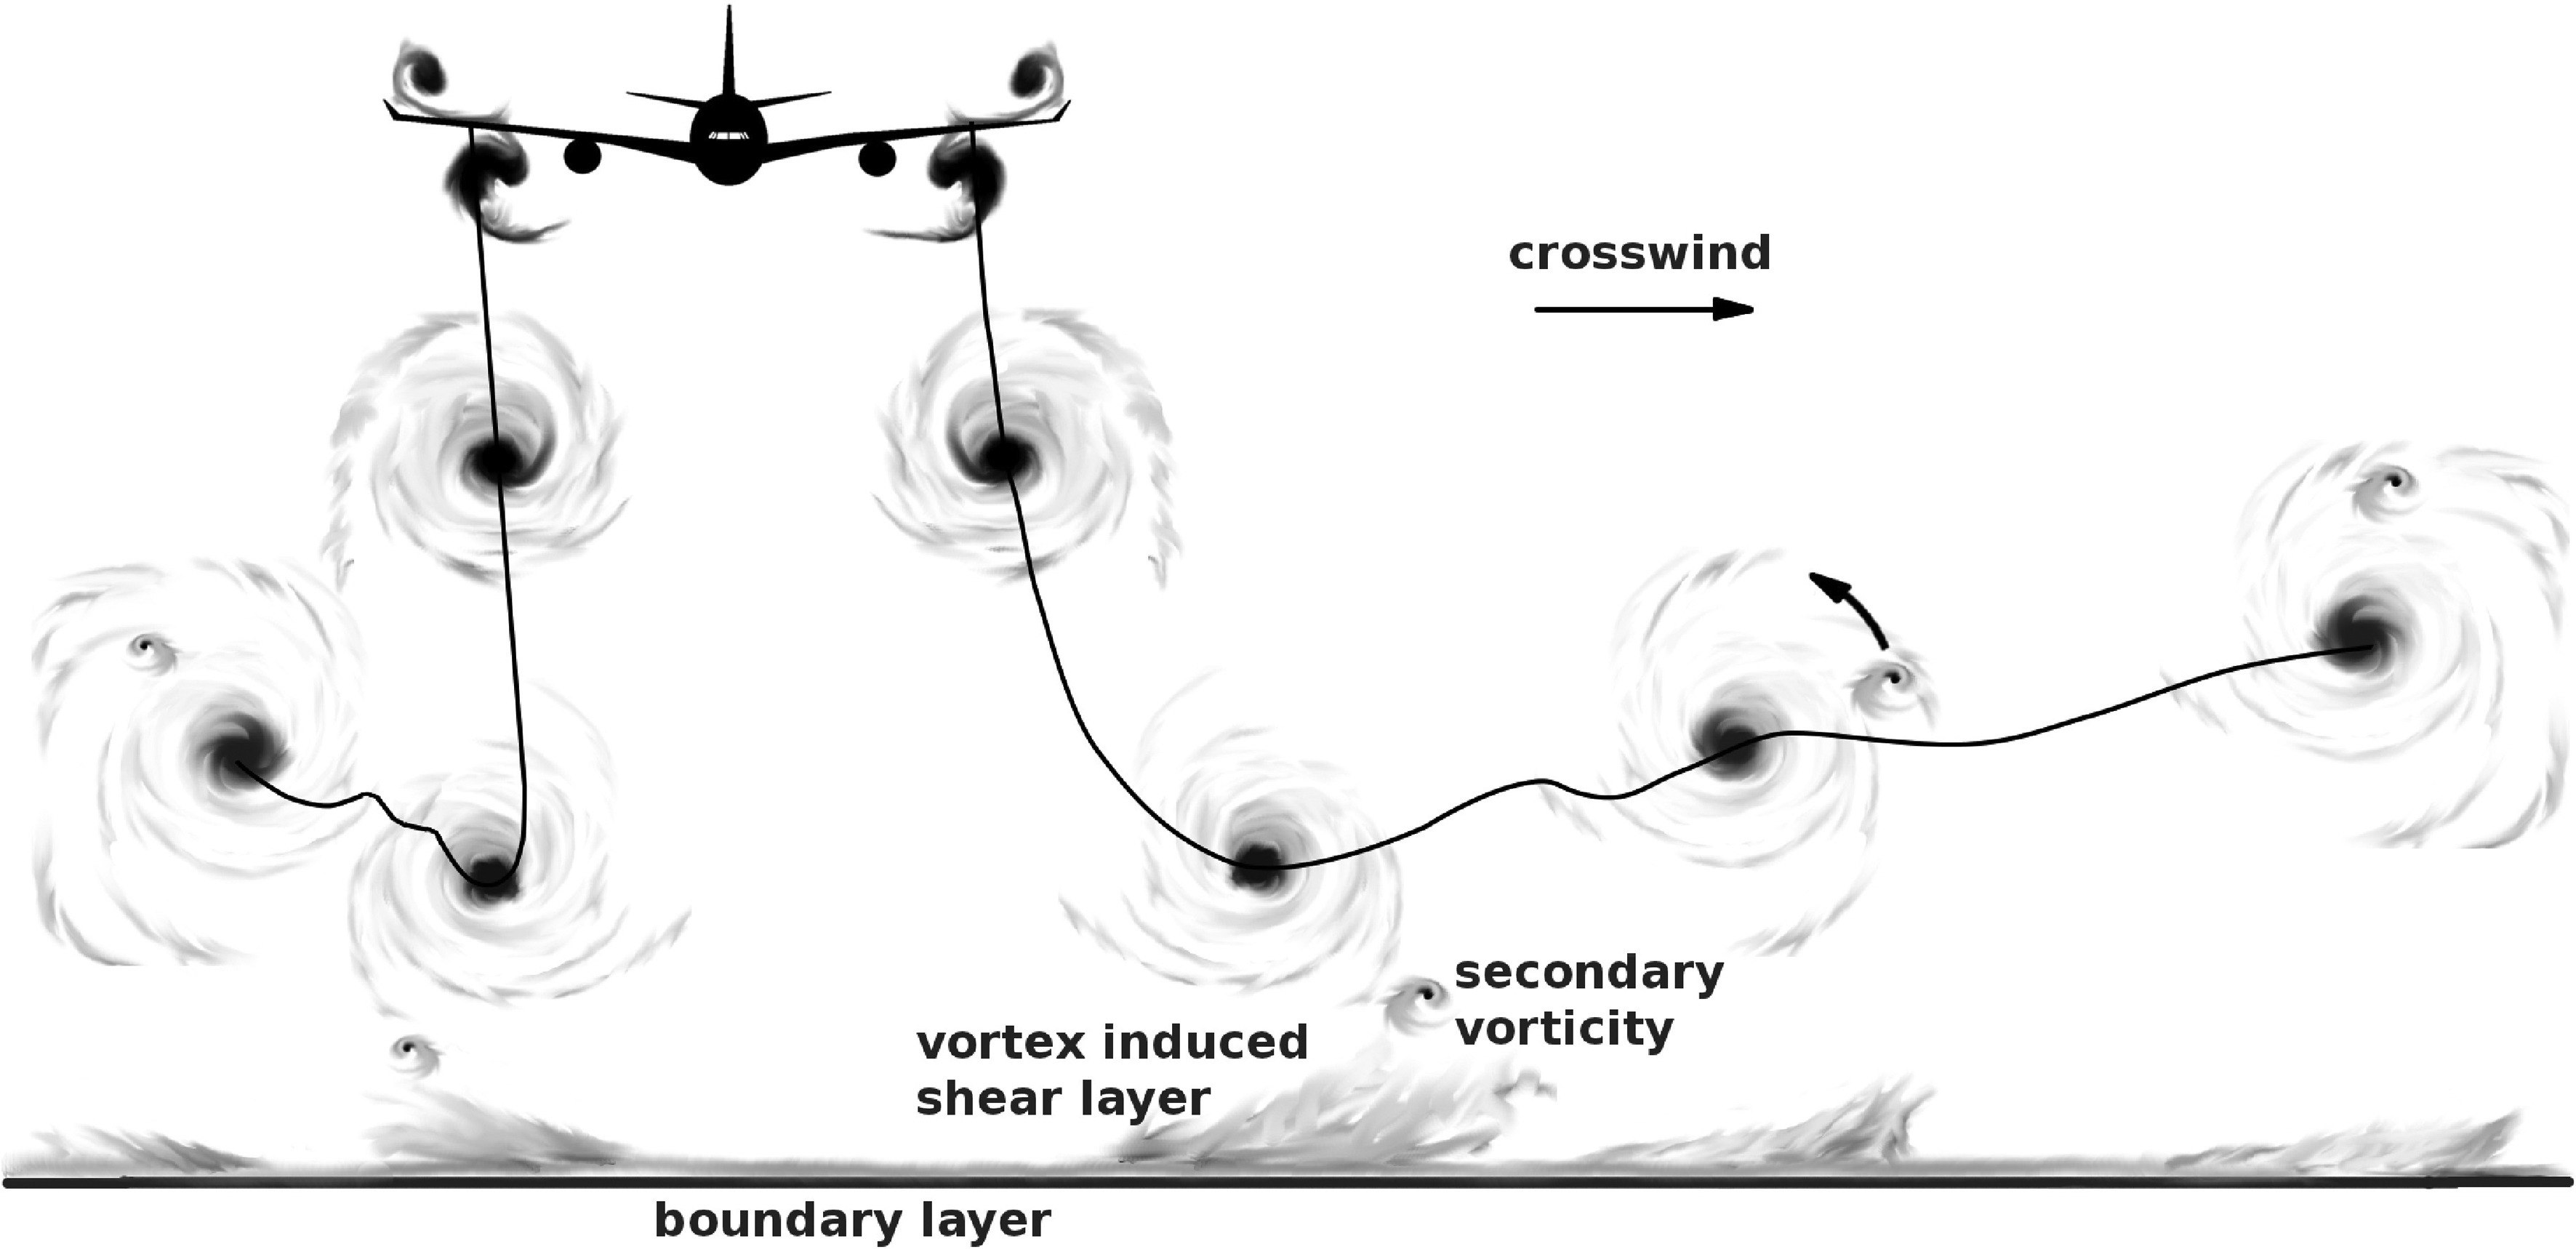
\includegraphics[width=0.8\textwidth]{graphics/Hallock_vortex_evolution.jpg}
    \caption[Wake vortex and ground effect]{Vortex evolution and ground effect~\cite[p. 29]{Hallock2018Apr}.} \label{fig:vortex_ground_effect}
\end{figure}


\subsection{Wake Vortex Separation}
An aircraft affected by the wake vortex can experience loss of lift or an induced rolling moment and velocity fluctuations (Figure~\ref{fig:vortex_encounter}).
This can lead to the up-set and potentially loss of control of an aircraft following the flight path of a preceding aircraft.
To diminish the effect of such vortices the trailing aircraft must be maintained at a safe distance behind the leading aircraft as the vortices spread laterally to either side of the flight path and are dissipated~\cite{Breitsamter2011Feb}.
The distance between aircraft pairs in view of safety is referred to as wake vortex separation. 

\begin{figure}[h]
    \centering
    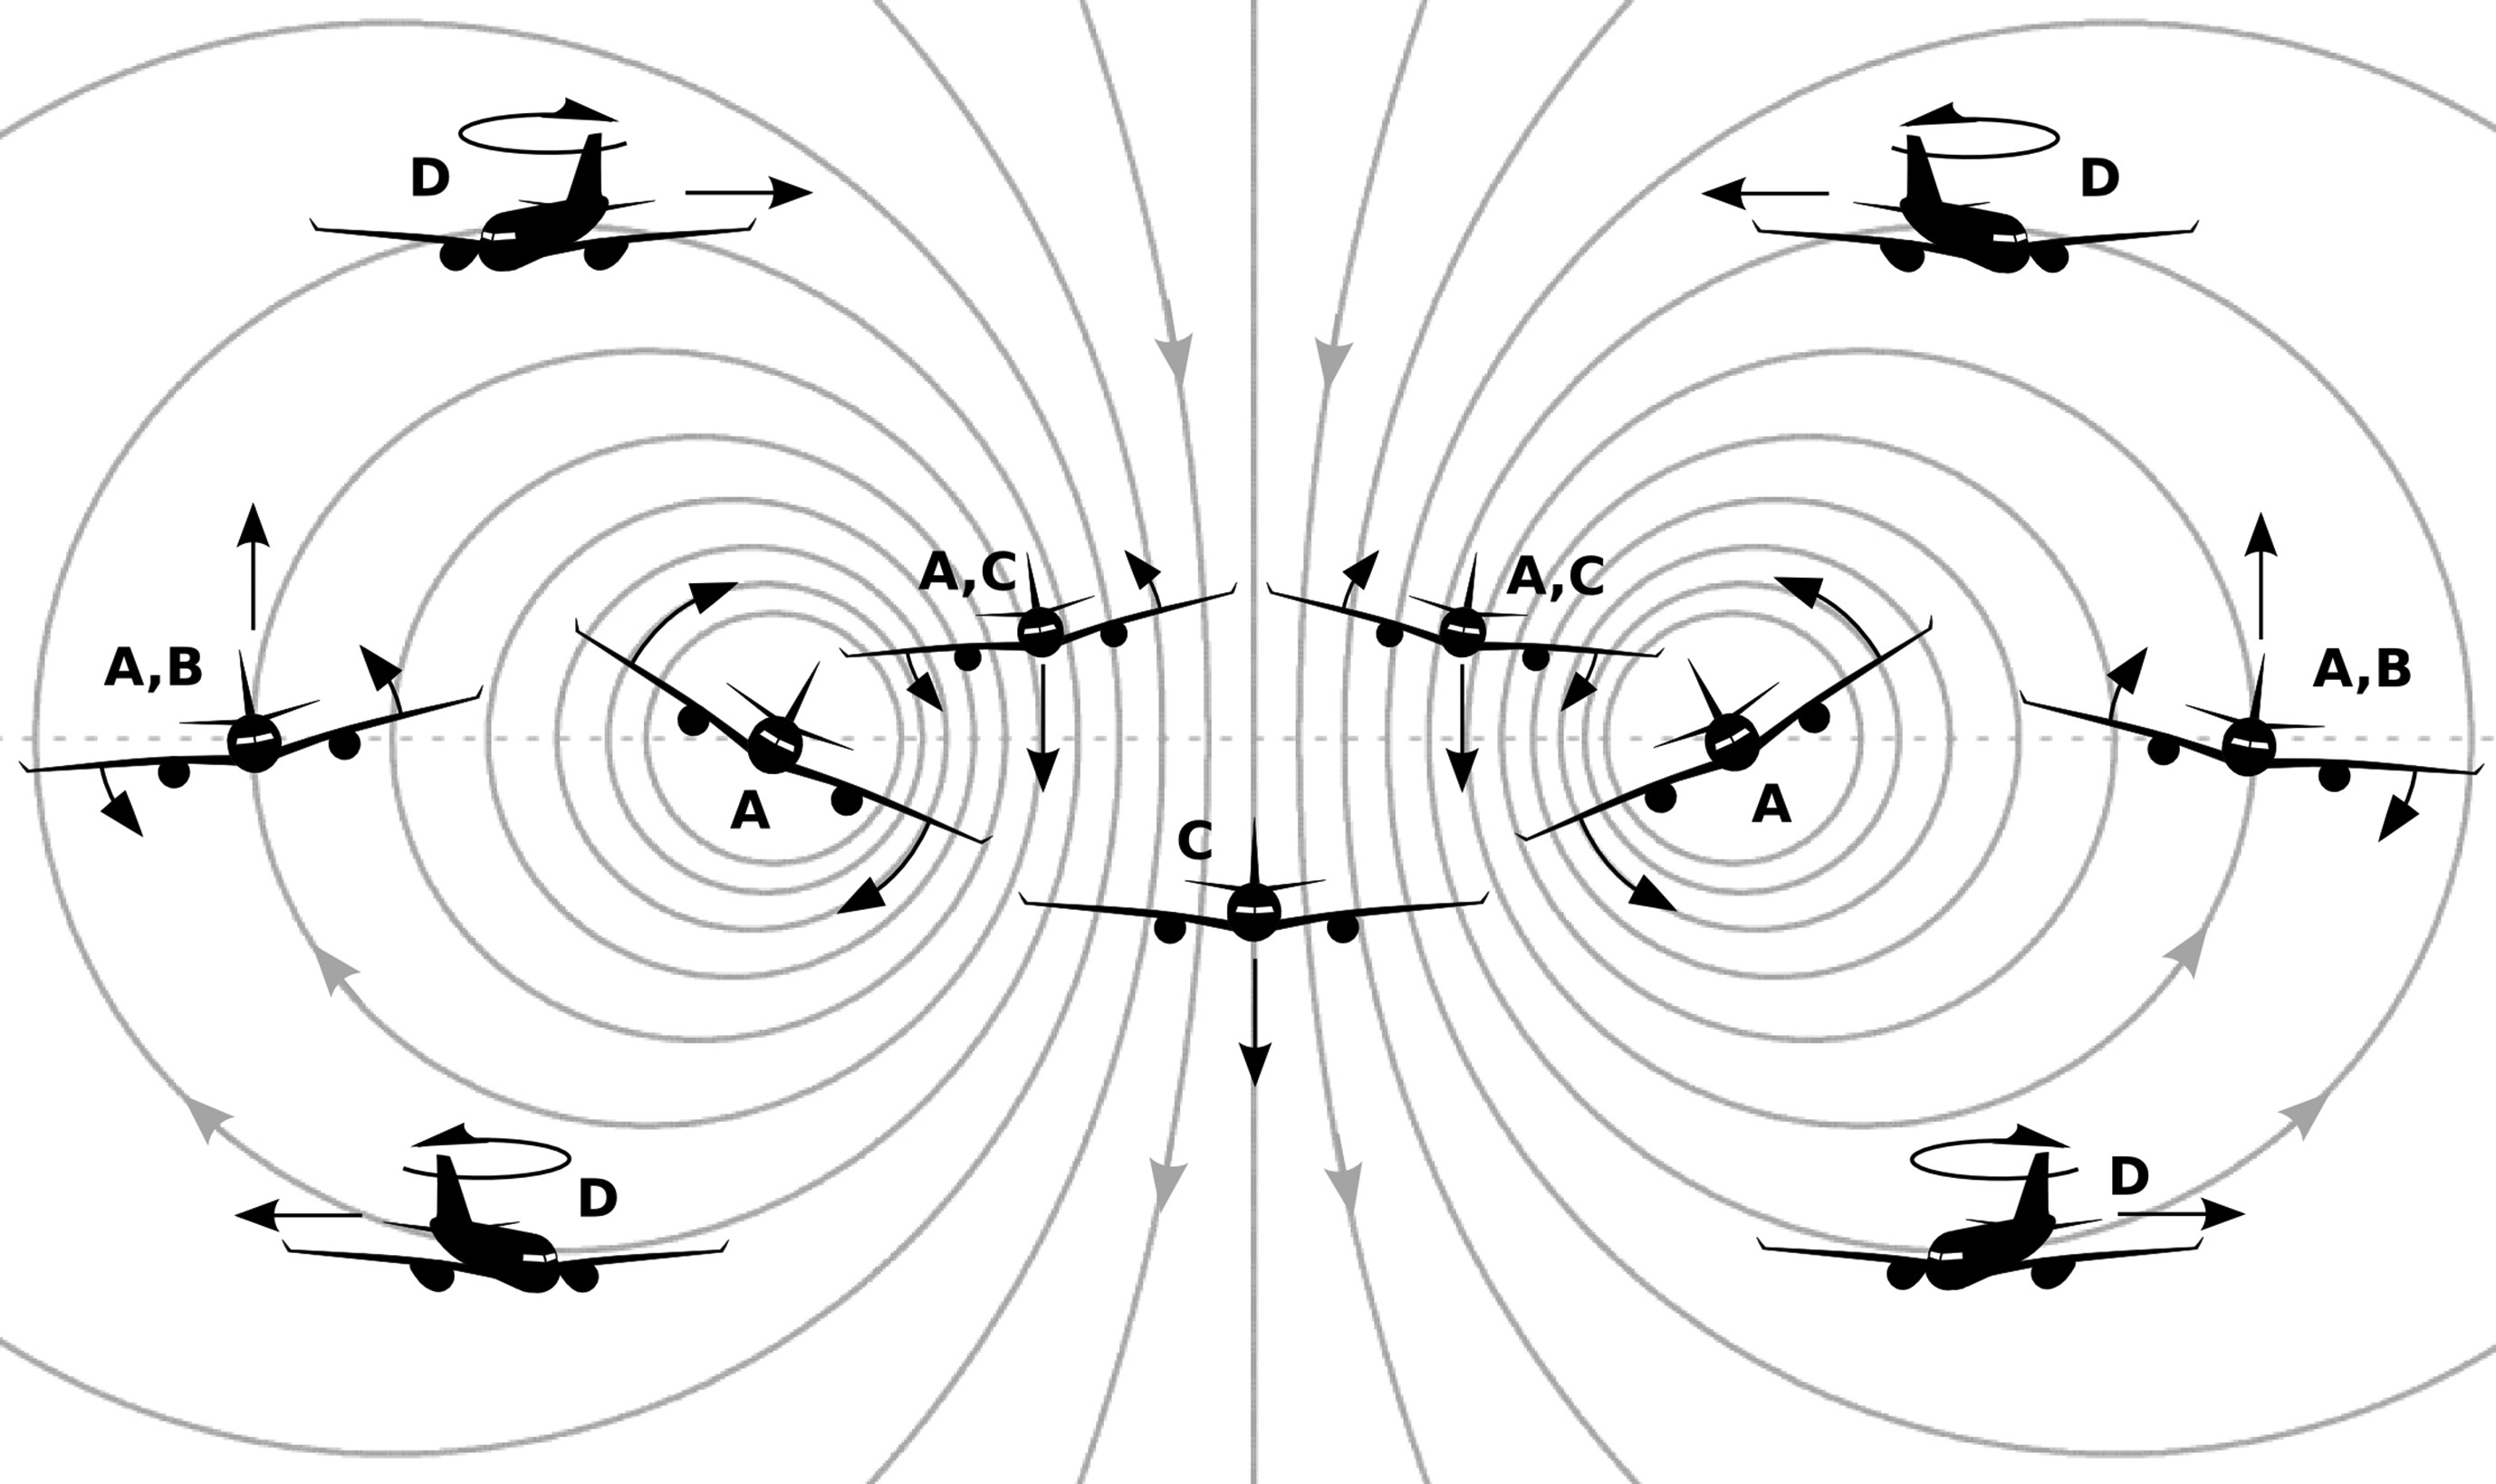
\includegraphics[width=0.8\textwidth]{graphics/reaction_in_wake.jpg}
    \caption[Wake vortex encounter]{Effect of wake vortex flow field on an aircraft. (A) induced rolling moment, (B) upward motion, (C) loss of lift~\cite[p. 33]{Hallock2018Apr}} \label{fig:vortex_encounter}
\end{figure}

Traditional separation standards, introduced in the seventies, are defined by ICAO  on the basis of certificated maximum take-off mass (MTOM) as shown in Table~\ref{tab:WTC}. The prescribed categories are three (i.e.Heavy, Medium and Light). In addition for aircraft in the order of $560000$~kg ICAO provides a subcategory to the Heavy types called Super Heavy. Some states have chosen to further increase the number of categories to adapt the wake turbulence categories (WTC) to specific airport requirements. Aerodromes in the UK split the Medium and Light categories each into two subcategories (Table~\ref{tab:WTC}), while the Federal Aviation Administration (FAA) places Boeing B757 into a separate category and increases the upper weight limit of the Light category.~\cite{icao_wtc, uk_aeronautical_information_services_wake_2017, noauthor_recat_2018}

\begin{table}[h]
    \centering
    \resizebox{1\textwidth}{!} {
    \begin{tabular}{l|c|c|c|c|c|c}
    ~    & \multicolumn{6}{c}{Category} \\ \hline
    ICAO & Super Heavy & Heavy (H) & \multicolumn{2}{c|}{Medium (M)} & \multicolumn{2}{c}{Light (L)} \\
    
    ~    & A380-800    & $ > 136000 $  & \multicolumn{2}{c|}{$ 136000-7000 $ } & \multicolumn{2}{c}{$ \leq 7000 $} \\ \hline
    
    ICAO (UK)   & ~  & Heavy (H) & Upper Medium (UM) & Lower Medium (LM) & Small (S)  & Light (L) \\
    
    ~    & A380-800    & $ > 136000 $  & $ 136000-104000 $     & $ 104000-40000 $      & $ 40000-17000 $ & $ \leq 17000 $   \\ \hline
    
    ICAO \& FAA (US)   & Super      & Heavy (H) & B757   & Large   & \multicolumn{2}{c}{Small} \\
    
    ~    & A380        & $ > 136000 $  & ~                 & $ 136000-18600 $      & \multicolumn{2}{c}{$ \leq 18600 $} \\ 
    \end{tabular}}
    \caption[ICAO wake turbulence categories based on maximum take-off mass]{ICAO wake turbulence categories based on maximum take-off mass (MTOM) in kg~\cite{icao_wtc, uk_aeronautical_information_services_wake_2017, kolos2013influence}.} \label{tab:WTC}
\end{table}

The ICAO wake turbulence categories (Table~\ref{tab:ICAO_WTC}) outline the worst case for each category and thus generate over-separation in many cases~\cite{noauthor_recat_2018}. The separation distances for instrumental flight rules are observed for the follower aircraft and are conventionally expressed in nautical miles (NM). The separation reverts to radar separation minimum (MRS) when wake turbulence restrictions are not required. As  prescribed  by  ICAO  the  horizontal MRS is 3~NM (or a reduced separation minimum of 2.5~NM may be applied under given conditions described in ICAO Doc 4444 PANS-AM~\cite{doc44444}), which translates to 79~s (66~s) time separation between leader and follower at final approach speed of 70~m/s.


% Please add the following required packages to your document preamble:
% \usepackage{multirow}
% \usepackage{graphicx}
\begin{table}[h]
\centering
\resizebox{\textwidth}{!}{%
\begin{tabular}{|c|c|c|c|c|c|}
\hline
\multicolumn{2}{|c|}{\multirow{2}{*}{ICAO WTC scheme}} & \multicolumn{4}{c|}{Follower}              \\ \cline{3-6} 
\multicolumn{2}{|c|}{}                                 & Super (A380-800) & Heavy & Medium & Light \\ \hline
\multirow{4}{*}{\rotatebox[origin=c]{90}{Leader}}       & Super (A380-800)       & (*)                & 6 NM  & 7 NM   & 8 NM   \\ \cline{2-6} 
                              & Heavy                  & (*)                & 4 NM  & 5 NM   & 6 NM   \\ \cline{2-6} 
                              & Medium                 & (*)                & (*)     & (*)      & 5 NM   \\ \cline{2-6} 
                              & Light                  & (*)                & (*)     & (*)      & (*)      \\ \hline
\end{tabular}%
}
\caption[ICAO wake turbulence categories and separation minima]{ICAO wake turbulence categories and separation minima to avoid wake vortex encounter~\cite{noauthor_recat_2018, rooseleer2015recat}.} \label{tab:ICAO_WTC}
\end{table}

It must be noted that the division of ICAO WTC into the RECAT scheme (Table~\ref{tab:RECAT-dist}) is not achieved by splitting each category in half.
The criteria used for categorisation of existing and new aircraft types are provided in detail in~\cite{rooseleer2015recat}. The case from the traffic mix at BIKF presents the arrangement shown in Table~\ref{tab:wtc2recat_division}. A more detailed illustration of the re-categorisation is presented in the upcoming section \ref{ssec:traffic_mix} on aircraft traffic mix (Figure~\ref{fig:post_fast_exit_mix_pie_v2}).

% Please add the following required packages to your document preamble:
% \usepackage{graphicx}
% \usepackage[table,xcdraw]{xcolor}
% If you use beamer only pass "xcolor=table" option, i.e. \documentclass[xcolor=table]{beamer}
\begin{table}[h]
\centering
\resizebox{0.7\textwidth}{!}{%
\begin{tabular}{clcllc}
\multicolumn{3}{c}{\cellcolor[HTML]{34CDF9}HEAVY} &  &  & \cellcolor[HTML]{FD6864}LIGHT \\ \hline
\multicolumn{1}{|c|}{\cellcolor[HTML]{34CDF9}CAT-A} & \multicolumn{1}{c|}{\cellcolor[HTML]{34CDF9}CAT-B} & \multicolumn{1}{c|}{\cellcolor[HTML]{32CB00}CAT-C} & \multicolumn{1}{c|}{\cellcolor[HTML]{F8FF00}CAT-D} & \multicolumn{1}{c|}{\cellcolor[HTML]{F8FF00}CAT-E} & \multicolumn{1}{c|}{\cellcolor[HTML]{FFC702}CAT-F} \\ \hline
\multicolumn{1}{l}{} &  & \multicolumn{4}{c}{\cellcolor[HTML]{F8FF00}MEDIUM}
\end{tabular}%
}
\caption{Transition from ICAO WTC to RECAT-EU categories. The categorisation process and criteria for assigning an existing aircraft type into RECAT-EU scheme is illustrated in detail in~\cite{rooseleer2015recat}}.
\label{tab:wtc2recat_division}
\end{table}

The noticeable changes in Table~\ref{tab:RECAT-dist} from Table~\ref{tab:ICAO_WTC} affect a follower aircraft, whose relative position from the ICAO scheme is shifted to the left in the new table after re-categorisation. Such benefit experiences for example a Heavy follower aircraft that is re-categorised as CAT-C, in which case the separation from the leader is reduced with up to 3 NM. 

%There is an RU logo in Figure~\ref{fig:ru-logo}.
%This logo will scale according to the width of the text on the page.

% Please add the following required packages to your document preamble:
% \usepackage{multirow}
% \usepackage{graphicx}
\begin{table}[h]
\centering
\resizebox{\textwidth}{!}{%
\begin{tabular}{|c|c|c|c|c|c|c|c|}
\hline
\multicolumn{2}{|c|}{\multirow{2}{*}{RECAT-EU scheme}} & \multicolumn{6}{c|}{Follower}                   \\ \cline{3-8} 
\multicolumn{2}{|c|}{}                                 & CAT\_A & CAT-B & CAT-C & CAT-D & CAT-E & CAT-F \\ \hline
\multirow{6}{*}{\rotatebox[origin=c]{90}{Leader}}            & CAT-A            & 3 NM   & 4 NM  & 5 NM  & 5 NM  & 6 NM  & 8 NM  \\ \cline{2-8} 
                                    & CAT-B            &    (*)    & 3 NM  & 4 NM  & 4 NM  & 5 NM  & 7 NM  \\ \cline{2-8} 
                                    & CAT-C            &    (*)    & (*)   & 3 NM  & 3 NM  & 4 NM  & 6 NM  \\ \cline{2-8} 
                                    & CAT-D            &    (*)    &   (*)    &    (*)   &   (*)    &   (*)    & 5 NM  \\ \cline{2-8} 
                                    & CAT-E            &    (*)    &   (*)    &   (*)    &   (*)    &   (*)    & 4 NM  \\ \cline{2-8} 
                                    & CAT-F            &    (*)    &   (*)    &    (*)   &   (*)    &   (*)    & 3 NM  \\ \hline
\end{tabular}%
}
\caption[RECAT-EU distance-based separation minima]{RECAT-EU WT distance-based separation minima on approach and departure. (*) means minimum radar separation (MRS), set at 2.5 NM, applicable as per current ICAO doc 4444 provisions \cite{doc44444, rooseleer2015recat, noauthor_recat_2018}.}
\label{tab:RECAT-dist}
\end{table}


\section{Runway Occupancy Time\label{sec:ROT}}

The Runway Occupancy Time (ROT) is defined by Eurocontrol as the amount of time that each aircraft occupies the runway~\cite{ROT_definition}. \\
This project focuses on Arrivals Runway Occupancy Time (AROT) in peak traffic hours, that is the time interval between the aircraft crossing the threshold and its tail vacating the runway~\cite{AROT_definition}. The threshold is the beginning of that portion of the runway that is available for landing.
The peak traffic hours are characterised by the time intervals when the airport operates at high load. High load interval or window is at least 15 minutes in length and has four or more flights arriving or departing from Keflavík Airport. The time between flights during the high load interval is set at $\leq$4~minutes (Figure~\ref{fig:Peak_Diagram}). This value is based on statistical data by Isavia in order to achieve two distinct peak hours: one in the morning and one in the afternoon. The last flight in a high load window that fulfils these requirements is not considered to be a part of the peak as its behaviour is not affected by an instantaneous next flight after it. The AROT metric is essential for the project because a following aircraft is not allowed to land on the same runway before it has been vacated by the leading aircraft. The interval to the next landing aircraft is specified as the Landing Time Interval (LTI) which is directly linked to the inter-arrival distance or in other words the wake turbulence separation.

\begin{figure}[h]
    \centering
    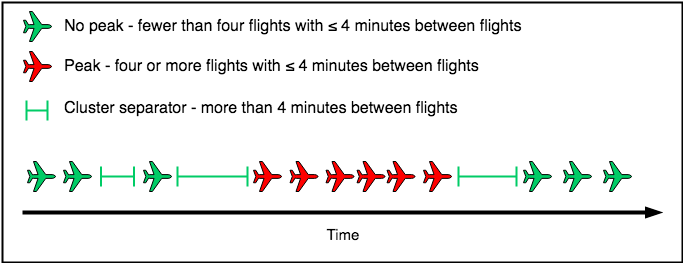
\includegraphics[width=1\textwidth]{graphics/Peak_Diagram.png}
    \caption[Rules defining a peak hour]{Rules used by Isavia to identify a high load interval as peak or not. The time separating each two aircraft in a peak cluster (red) is set as less than or equal to 4 minutes. The last red aircraft in the peak cluster is not counted as part of the peak. Cluster separators are defined as time intervals larger than four minutes.}
    \label{fig:Peak_Diagram}
\end{figure}


\section{Runway Capacity\label{sec:runway_capacity}}

ICAO generally defines airport capacity as the number of movements per unit of time that can be accepted during different meteorological conditions~\cite{airport_capacity_methodology}. 
Several measures are currently used to estimate the amount of aircraft movements on the runways of an airport in a specified time interval.
R. de Neufville~\cite{de_neufville_airport_2013} states that the capacity of runway systems determines the ultimate capacity of an airport and that its principal measure maximum throughput capacity. It indicates the average number of movements that can be performed on the runway system in one hour in the presence of continuous demand, while adhering to all the separation requirements imposed by the air traffic management (ATM) system~\cite{de_neufville_airport_2013}.
The Capacity Envelope method used by Isavia to estimate the throughput capacity at BIKF takes into consideration the number of arrivals and departures within a selected time frame. This approach allows to measure the throughput capacity and model the maximum possible values or the potential of the airfield. A summary of the capacity envelope for a period of one year is shown in Figure~\ref{fig:capacity_evnelope} for a 15~minute time interval. 

\begin{figure}[h]
    \centering
    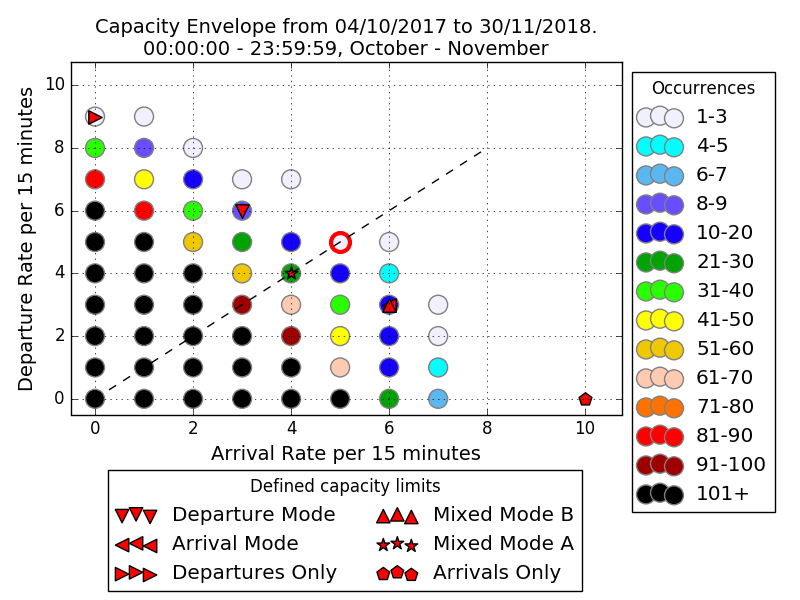
\includegraphics[width=0.8\textwidth]{graphics/fig_Capacity_Envelope_2017-10-04_to_2018-11-30_15min_occurrences_limits.png}
    \caption[Capacity envelope for BIKF]{Capacity envelope at BIKF since October 2017. The measured time interval is 15 minutes and includes both the morning and afternoon peaks. The capacity limits of the airfield are also defined and noted on the figure for various sequence modes. The mixed modes indicate equal arrivals and departures (Mixed~Mode~A) or two times more arrivals than departures (Mixed Mode B), the later being a tendency during the afternoon peaks. The figure is from Isavia´s internal GUI Víkingaskipið.}  \label{fig:capacity_evnelope}
\end{figure}

This approach indicates a maximum measured capacity of four arrivals to four departures in a "Mixed~Mode~A". This equilibrium mode is defined as the primary measure for the throughput capacity of BIKF. The values are in accord with the defined peak hour intervals in the previous section~\ref{sec:ROT}

There are many aspects of a runway system that can affect the number of aircraft that can land or depart from an airfield and some of those are listed bellow~\cite{de_neufville_airport_2013, kim_validation_2010}.
\begin{itemize}
    \item Number and geometric layout of the runways.
    \item State and performance of the ATM system.
    \item Separation requirements between aircraft pairs imposed by the ATM.
    \item Weather conditions (visibility, precipitation, cloud ceiling). 
    \item Wind direction and strength.
    \item Mix of aircraft using the airport.
    \item Sequence of movement on each runway (arrivals - departures split)
    \item Type and location of taxiway exits from the runway.
    \item Runway occupancy time.
    \item Controller workload.
    \item Noise-related constraints and other environmental considerations.
\end{itemize}

Two of the above mentioned factors are principal in determining airfield capacity, namely the wake vortex separation requirements and runway occupancy~\cite{kolos2013influence}. Those are in turn influenced by traffic mix, seasonal factors and runway exits, to mention a few. The following chapter~\ref{cha:methods} on Methods  will deal with some of those aspects. 

\fxnote{equipment specifications in the tower that might influence the WTC separtarion decision-talk to Haraldur, Talk to Hjalti about the 2,5~-~3~NM MRS issue!}

\section{Runway Occupancy and Landing Time Interval Study Objective}\label{sec:study_objective}
The goal of examining the arrival runway occupancy times and the landing time intervals (LTI) is to determine whether the implementation of the RECAT-EU scheme at BIKF under certain conditions, would affect the throughput of the airfield. 
LTI is the a measure of the time separation between aircraft pairs derived from the distance separation between the aircraft and the final approach speed (time travelled is distance travelled divided by velocity).
% The LTI is directly influenced by the distance separation of arrival pairs and the final approach speed of the aircraft .
Additionally the analysis could indicate whether the limiting element is the runway occupancy or the separation requirement. The proposed transition by Eurocontrol from ICAO WTS to RECAT-EU scheme suggests a decrease in distance separation for a number of the aircraft pairs (Table~\ref{tab:delta_distance_wtc2recat}).

% Please add the following required packages to your document preamble:
% \usepackage{multirow}
% \usepackage{graphicx}
\begin{table}[h]
\centering
\resizebox{\textwidth}{!}{%
\begin{tabular}{|c|c|c|c|c|c|c|c|}
\hline
\multicolumn{2}{|c|}{}                                          & \multicolumn{6}{c|}{Follower}                                                                                                                                                                                                   \\ \cline{3-8} 
\multicolumn{2}{|c|}{\multirow{-2}{*}{RECAT-EU scheme}} & CAT-A                             & CAT-B                                & CAT-C                         & CAT-D                         & CAT-E                         & CAT-F                                                \\ \hline
                                                        & CAT-A & \cellcolor[HTML]{FD6864}(+0,5 NM) & \cellcolor[HTML]{67FD9A}-2 NM        & \cellcolor[HTML]{67FD9A}-1 NM & \cellcolor[HTML]{67FD9A}-2 NM & \cellcolor[HTML]{67FD9A}-1 NM &                                                      \\ \cline{2-8} 
                                                        & CAT-B &                                   & \cellcolor[HTML]{67FD9A}-1 NM        &                               & \cellcolor[HTML]{67FD9A}-1 NM &                               & \cellcolor[HTML]{FD6864}+1 NM                        \\ \cline{2-8} 
                                                        & CAT-C &                                   & \cellcolor[HTML]{67FD9A}-1 (-1,5) NM & \cellcolor[HTML]{67FD9A}-1 NM & \cellcolor[HTML]{67FD9A}-2 NM & \cellcolor[HTML]{67FD9A}-1 NM &                                                      \\ \cline{2-8} 
                                                        & CAT-D &                                   &                                      &                               &                               &                               &                                                      \\ \cline{2-8} 
                                                        & CAT-E &                                   &                                      &                               &                               &                               & \cellcolor[HTML]{67FD9A}{\color[HTML]{000000} -1 NM} \\ \cline{2-8} 
\multirow{-6}{*}{\rotatebox[origin=c]{90}{Leader}}                                & CAT-F &                                   &                                      &                               &                               &                               & \cellcolor[HTML]{FD6864}(+0,5 NM)                    \\ \hline 
\end{tabular}%
}
\caption[Difference in wake separation minima on approach between reference ICAO and RECAT-EU schemes]{Difference in wake separation minima on approach between reference ICAO and RECAT-EU schemes (full proposal)~\cite{rooseleer2015recat}}
\label{tab:delta_distance_wtc2recat}
\end{table}



% % Please add the following required packages to your document preamble:
% % \usepackage{multirow}
% % \usepackage{graphicx}
% \begin{table}[]
% \centering
% \resizebox{\textwidth}{!}{%
% \begin{tabular}{|c|c|c|c|c|c|c|c|}
% \hline
% \multicolumn{2}{|c|}{}                                          & \multicolumn{6}{c|}{Follower}                                                                                                             \\ \cline{3-8} 
% \multicolumn{2}{|c|}{\multirow{-2}{*}{RECAT-EU scheme}} & CAT-A & CAT-B                        & CAT-C & CAT-D                        & CAT-E                        & CAT-F                        \\ \hline
%                                                         & CAT-A &       & \cellcolor[HTML]{67FD9A}-20s &       & \cellcolor[HTML]{67FD9A}-40s & \cellcolor[HTML]{67FD9A}-20s &                              \\ \cline{2-8} 
%                                                         & CAT-B &       &                              &       & \cellcolor[HTML]{67FD9A}-20s &                              & \cellcolor[HTML]{FD6864}+20s \\ \cline{2-8} 
%                                                         & CAT-C &       &                              &       & \cellcolor[HTML]{67FD9A}-40s & \cellcolor[HTML]{67FD9A}-20s &                              \\ \cline{2-8} 
%                                                         & CAT-D &       &                              &       &                              &                              &                              \\ \cline{2-8} 
%                                                         & CAT-E &       &                              &       &                              &                              & \cellcolor[HTML]{67FD9A}-20s \\ \cline{2-8} 
% \multirow{-6}{*}{Leader}                                & CAT-F &       &                              &       &                              &                              & \cellcolor[HTML]{FD6864}+20s \\ \hline
% \end{tabular}
% }
% \caption[Time difference between reference ICAO and RECAT-EU schemes]{Time difference in wake separation on departure between reference ICAO and RECAT-EU schemes(full proposal) \cite{rooseleer2015recat}}
% \label{tab:delta_times_wtc2recat}
% \end{table}

The implementation of RECAT shifts the wake separation minima for arrival and departure pairs thus creating the potential for reduced time separation between the aircraft. The reduction of the time interval between landings facilitates increas in the throughput capacity of the runways. 
Figure~\ref{fig:AROT_LTI_rwy19_H_M} may be used to illustrate the hypothesis. The current ICAO time separation reference, indicated by the red vertical line for BIKF RWY-19 will be relocated to the left for some of the aircraft pairs under the RECAT scheme. This relocation will be more noticeable for RECAT C-C and C-D pairs formed from the ICAO HEAVY-MEDIUM pairs, in which case the separation is reduced from 5 NM to 3 NM. A shift of the reference separation line creates the potential for shift in the distribution of the LTI, as long as it does not overlap with the ROT. Furthermore study on the runway capacity of significantly larger airports~\cite{kolos2013influence} suggests that the frequency distribution of LTI tends to compress or squeeze to the right of the reference line with less standard deviation about the mean when the air traffic is intensified.

\begin{figure}[h]
    \centering
    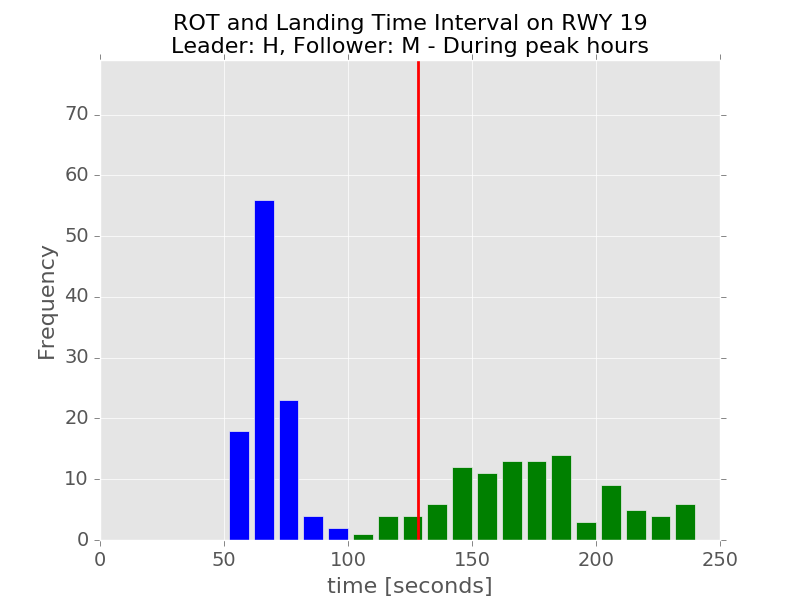
\includegraphics[width=0.8\textwidth]{graphics/fig_rot_landig_time_interval_RWY19_leader_H_follower_M_peak-hour_BAR_20171004_20181130.png}
    \caption[Caption table]{Arrival runway occupancy time (blue) and landing time intervals (green) for Heavy leader - Medium follower pairs on BIKF runway RWY-19. The observed time period is from October 2017 to November 2018. The red line indicates the ICAO WTC reference time separation for the selected H-M aircraft pairs. The figure is from the Isavia´s internal GUI Víkingaskipið.}\label{fig:AROT_LTI_rwy19_H_M}
\end{figure}




%%% Local Variables: 
%%% mode: latex
%%% TeX-master: "DEGREE-NAME-YEAR"
%%% End: 
%%RUM: Introduction


\chapter{Methods\label{cha:methods}}
Data collection on flights passing through the airspace monitored and controlled by Isavia has been going on for several years now. This data is filtered and stored on company servers for reference and analysis. The statistical analysis for this project was done in Python and used to determine the fleet mix at BIKF, runway occupancy and landing intervals.

\section{Data Collecting and Data Filtering}
More detailed data collection commences on 21 November 2014 with the implementation of the Automatic Dependent Surveillance-Broadcast (ADS-B) system by Isavia. ADS-B was preferred to radar at Keflavik International Airport because of improved signal accuracy~\cite{isavia_wiki}. The ADS-B equipped aircraft through Keflavik Airport are estimated to be around~$90\%$~\cite{isavia-rounardeild_rannsoknir_2018}. The aircraft surveillance data specifications used for measurements are in the Eurocontrol ASTERIX Category 21 standard~\cite{ASTERIX_ADS-B_specs}.
The reading from the position of the ADS-B antenna of the aircraft is used instead of the tail and nose positions. This simplification could result in a few seconds difference. Certain filtering of the ADS-B data is applied before commencing measurements and calculations~\cite{isavia_wiki}: 
\begin{itemize}
    \item All records with no latitude, longitude and/or time data are omitted.
    \item The records are filtered with regards to quality, i.e. filtered with regards to Target Surveillance status, MOPS version, NUC/NIC, NACp, SIL and PIC.
    \item An ADS-B data record within 0.5 second from another is omitted, i.e. if there are less than 0.5 seconds between two successive locations one of the records is omitted.
    \item An algorithm is used to analyse the data and determine if it originates from two different flights (the flight stops for 15 minutes or more after/before taxiing). If so the data for the second flight is omitted
    \item The velocity is calculated from ADS-B location data and ADS-B time data (velocity = distance travelled/time). The ADS-B velocity record is optional in the ASTERIX category 21 standard and is therefore unreliable in measurements. Since the velocity is calculated from measured data, it can exhibit spikes. To get a more realistic velocity curve, a Savitzky-Golay filter is applied to smooth the data.
    \item An aircraft main gear lift-off is considered to be the point where the ADS-B ground bit is removed, i.e. the ADS-B ground bit goes from a value of 1 to a value of 0.
    \item An aircraft touchdown is considered to be the point where the ADS-B ground bit is set, i.e. the ADS-B ground bit goes from a value of 0 to a value of 1.
    \item An aircraft is considered to be stationary when the velocity is below 0.5~knots and to be moving if the velocity is greater than 0.5~knots.
    
\end{itemize}

\fxnote{The ROT measurements have been checked by: comparing them to measurements made by hand.
Who measures and who checks them and how???}

\section{Data Manipulation}
The data was obtained from the database using SQL server and stored as csv files. The manipulations on the data frames were performed using the functionality of Pandas and NumPy data analysis tools and computing packages for Python. A key table containing information about 2300 aircraft models, including ICAO and RECAT-EU wake turbulence categories for each model, was also used as reference. 
The reference table was provided by Eurocontrol. 
The Isavia aircraft data was cross-referenced with the Eurocontrol key table based on ICAO aircraft type labels, the mutual characteristic in both data sets. 
After cross-referencing a RECAT-EU category was assigned to each of the aircraft arriving at BIKF in peak hours. Outliers bellow the 0,003~quartile and above the 0,997~quartile were regarded as anomalies and removed from the data-set, based on AROT values. 
The resulting data frame was used for initial analysis in this project. 
It contained over 11500 arrivals for the time period of almost four years (from 01.01.2015 until 30.11.2018). The data frame contained unique information about the AROT of each aircraft, landing time and runway, along with the ICAO wake category. Consequently the time frame for the analysis was reduced to 13 months (from 04.10.2017 to 30.11 2018) because of the effect of fast-exits on AROT, which is explained in the upcoming section \ref{sssec:runway_usage_arot}


\subsection{Aircraft Traffic Mix\label{ssec:traffic_mix}}
The aircraft traffic mix is one of the components that affect runway capacity as mentioned in Section~\ref{sec:runway_capacity}. Sorting the aircraft fleet arriving at BIKF into ICAO WTC reveals that the majority of flights~(85,4\%) are in the Medium wake category (Figure~\ref{fig:post_fast_exit_mix_pie_v2}) and the rest are mainly in the Heavy category~(14,2\%) with less than one percent Light aircraft. The small portion of Light flights can be explained with the policy of ATM at BIKF to avoid servicing those flights during the morning and afternoon peaks. This distribution of the three categories implies that combining the aircraft into arriving pairs would produce primarily Medium-Medium pairs. This is confirmed by the analysis of the number of arrival pairs in the ICAO categories (Table~\ref{tab:pairs_mix_to_wtc}).\\
When this same fleet is presented using the RECAT categories, the prevailing category is CAT-C (73,7\%), followed by CAT-D (22,1\%). The percentage of each of the remaining categories varies within 2\%. The expectation that this distribution of the RECAT categories would result in primarily in C-C pairs is confirmed later on by the analysis presented in Table~\ref{tab:pairs_mix_to_recat}. \\
The method of of re-categorising the traffic mix is a prerequisite for assembling the RECAT pairs later on and determining the main aircraft categories that will be considered for analysis along with estimating the inter arrival distances characteristic of each pair.
\begin{figure}[h]
    \centering
    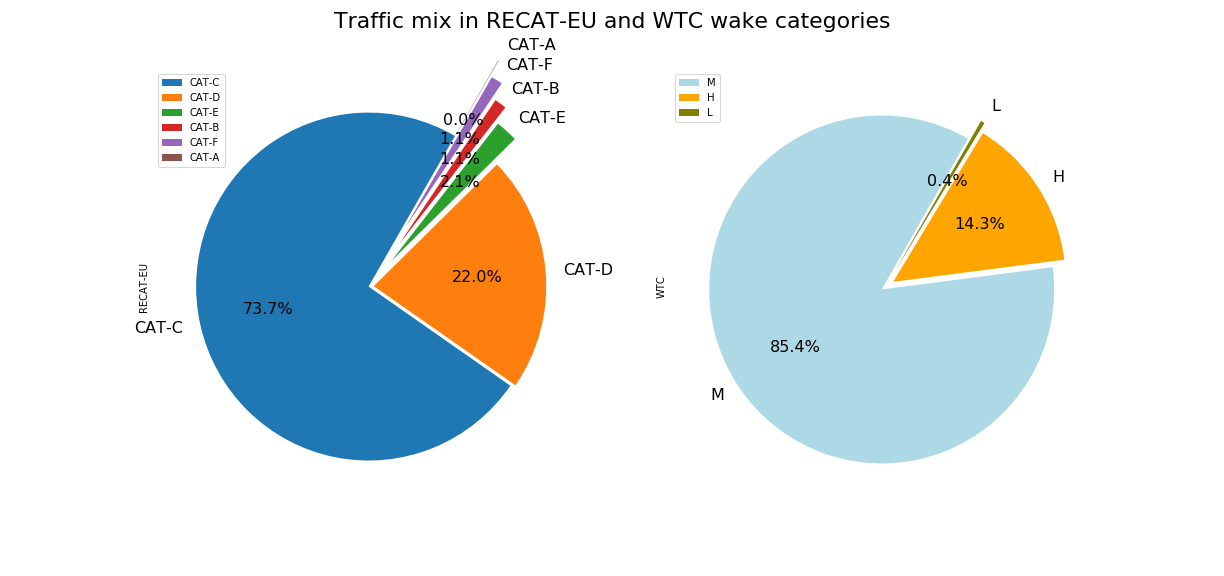
\includegraphics[width=1\textwidth]{graphics/fig_post_fast_exit_mix_pie_v2.png}
    \caption[Traffic mix in RECAT-EU and ICAO WTC]{The traffic mix at Keflavik Airport represented in RECAT-EU categories alongside ICAO WTC categories.}
    \label{fig:post_fast_exit_mix_pie_v2}
\end{figure}
Another approach for classification of the traffic fleet mix at BIKF in peak hours is to identify the aircraft types or models. The traffic data contains ICAO aircraft type designator, that is a two-, three- or four-character code comprising of numbers and letters. This designator is unique for each aircraft type. The top fifteen ICAO types of the aircraft mix are presented in Figure~\ref{fig:traffic_mix_by_model}. Dominating the scene (56.8\% of all arrivals) is the Boeing~757-200 model (ICAO:B752), followed by the Boeing~767-300 (ICAO:B763).
\begin{figure}[h]
    \centering
    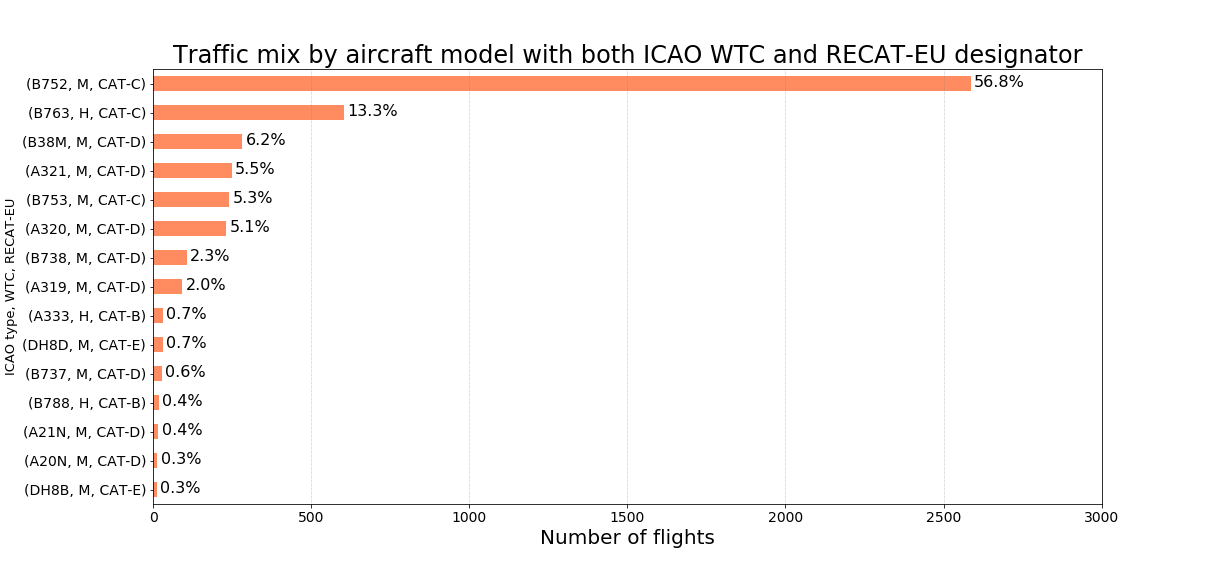
\includegraphics[width=1\textwidth]{graphics/fig_traffic_mix_by_model.png}
    \caption[Traffic mix by aircraft model.]{The traffic mix at Keflavik Airport grouped by aircraft type are shown alongside the ICAO WTC and RECAT-EU designators. The top three models comprise the major part of the Icelandair fleet.}
    \label{fig:traffic_mix_by_model}
\end{figure}
 Those models represent a major part of the Icelandair fleet and the share of the Boeing~737~MAX~8 (ICAO:B38M) is likely to increase as the Icelandair company plans to gradually add sixteen new B38M and B39M models from the beginning of 2018~\cite{icelandair_fleet}. The aircraft types are shown with their ICAO and RECAT categories and the tendency is towards increasing the share of the Medium-Medium pairs, or the C-D and D-C RECAT pairs respectively, with the addition of the new Icelandair aircraft.

% -----------------------

\subsection{Arrival Runway Occupancy Time Considerations}\label{ssec:AROT_considerations} 

The ICAO Doc 4444 PANS-AM~\cite{doc44444} dictates that the radar separation minimum (MRS) between succeeding aircraft which are established on the same final approach track, may be reduced from 3~NM to 2,5~NM under certain conditions. One of the requirements is that the average runway occupancy time of landing aircraft is proven, by means such as data collection and statistical analysis and methods based on theoretical model, not to exceed 50 seconds. 

\subsubsection{Traffic Mix and AROT\label{sssec:mix_effect_arot}}
Several approaches were used to look at the AROT at the airfield. First the runway occupancy was inspected based on the RECAT category of the aircraft (Figure~\ref{fig:RECAT_AROTs_boxplot}). 
\begin{figure}[h]
    \centering
    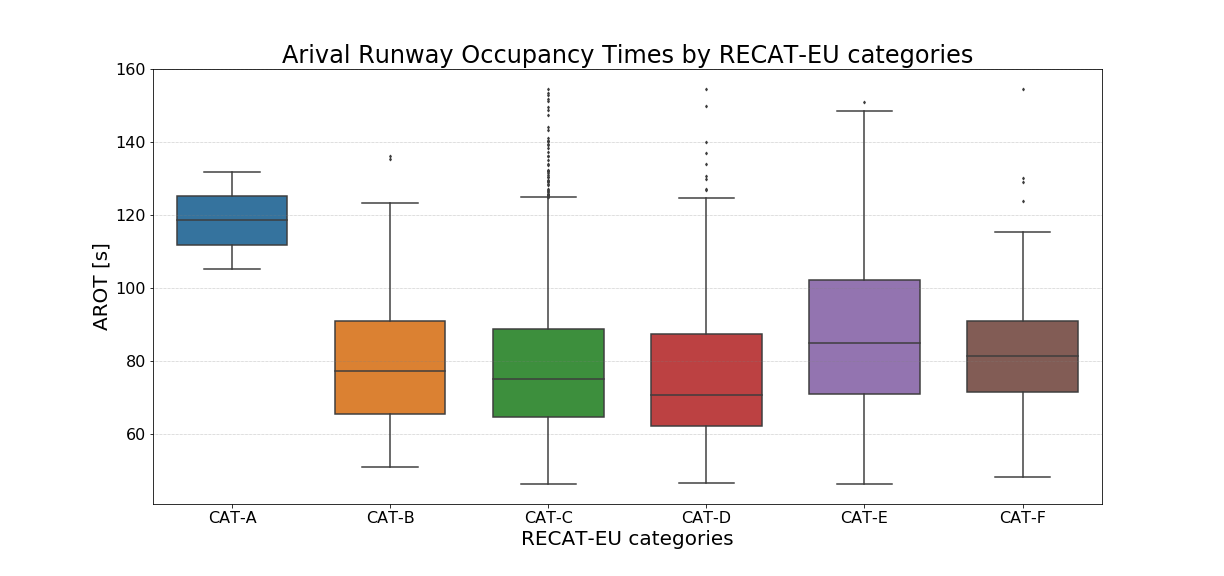
\includegraphics[width=1\textwidth]{graphics/fig_RECAT_AROTs_boxplot.png}
    \caption[AROTs box-plot for RECAT categories, all runways]{Arrival Runway Occupancy Times for the different RECAT-EU categories based on data gathered for a period of one year since October 2017. The coloured blocks indicate where 50\% of the data are or the inter-quartile range (IQR); lower edge is the 25\textsuperscript{th}~percentile, upper edge is the 75\textsuperscript{th}~percentile. The whiskers are at $\pm$1,5$\times$IQR  The box plot shows the AROTs for all runways at BIKF.}
    \label{fig:RECAT_AROTs_boxplot}
\end{figure}
The analysis showed that none of the average runway occupancy values fulfils the 50~seconds limit for reduced MRS. Closest to the required time were the aircraft from the CAT-D and CAT-C with mean values of 75 and 78 seconds respectively (Table~\ref{tab:AROT_RECAT_stats}). Those results point to the necessity of setting the MRS reference value at 3 NM and also suggest that the runway occupancy will be a limiting factor for the cases in which MRS is applicable (Table~\ref{tab:RECAT-dist}). This limitation is also confirmed by the statistical analysis for each of the runways in the following sections.% \ref{sssec:seasonal_arot}, \ref{sssec:runway_usage_arot}. 

\subsubsection{Seasonal Variation of AROT\label{sssec:seasonal_arot}}
Another approach was to analyse the seasonal variations of the runway occupancy. The differentiation between summer and winter months was based on AROT for a period of one year (Table~\ref{tab:month2season_arot}). Months with average AROT~$\leq$80~seconds formed the summer season and the rest were selected as winter months. This separation is purely subjective but succeeds in forming two seasons with equal number of months. On average the seasonal variation of runway occupancy times was eight seconds as seen in Table~\ref{tab:summer_winter_arot}. Sill the seasonal variation should be taken into consideration as they can effect the AROT significantly, especially in the winter months when adverse weather conditions could impair the runway surface by accumulated slush, snow or ice, thus diminishing braking action. Good braking action due to runway surface condition is also one of the requirements for reduced MRS as provided by~\cite{doc44444}.
% Please add the following required packages to your document preamble:
% \usepackage{graphicx}
\begin{table}[h]
\centering
\resizebox{0.8\textwidth}{!} & \multicolumn{1}{l|}{50\%} & \multicolumn{1}{l|}{75\%} & \multicolumn{1}{l|}{max} \\ \hline
\multicolumn{1}{|l|}{SUMMER} & \multicolumn{1}{r|}{3727} & 76  & 17 & 46 & 63  & 72 & 87  & 155 \\ \hline
\multicolumn{1}{|l|}{WINTER} & \multicolumn{1}{r|}{937}  & 84  & 20 & 45 & 69  & 84 & 96  & 153 \\ \hline
\end{tabular}%
}
\caption[AROTs for the air traffic mix by season]{AROT statistics for the air traffic mix at KEF by season. The count is the number of landings in peak hours since October 2017}
\label{tab:summer_winter_arot}
\end{table}

\subsubsection{Runway Usage and AROT\label{sssec:runway_usage_arot}}
Runway occupancy for each of the runways was also examined both with regards to seasonal variations and fast-exit usage. The usage of the four runways in peak hours is shown in Figure~\ref{fig:runway_usage_peak}. 
\begin{figure}[h]
    \centering
    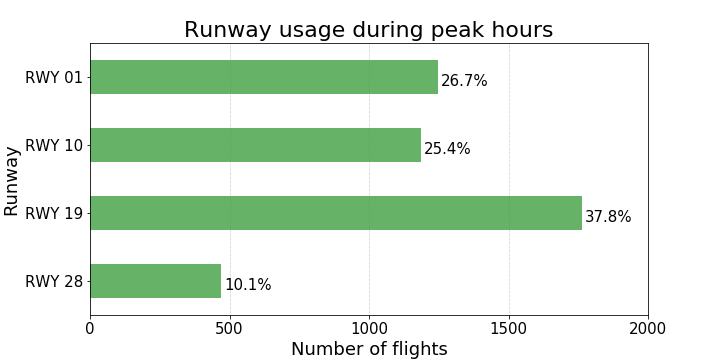
\includegraphics[width=0.8\textwidth]{graphics/fig_runway_usage_peak.png}
    \caption[Runway usage at BIKF during peak hours]{Runway usage at BIKF during peak hours for a period of one year. RWY-19 is the preferred runway, followed by RWY-01 and RWY-10. The RWY-01 is equipped with fast-exit TWY~A-1 and RWY-28 with fast-exit TWY~B-1.}
    \label{fig:runway_usage_peak}
\end{figure}
BIKF airfield is equipped currently with two fast-exit taxiways designated as TWY~A-1 and TWY~B-1. The first was completed on 26~July,~2017 and the later on 4~October,~2017. The date A-1 became operational was chosen as the beginning for the data set considered for analysis in this project. The reason behind this is the beneficial effect that fast-exits have on reducing arrival runway occupancy time. Taxiway A-1 provides a fast-exit track to the left for RWY-01, in the south-north landing direction, and B-1 serves RWY-28 exiting to the right in the east-west direction. The statistical analysis points to decreased AROT on average for RWY-01 after the start of A-1 (Table~\ref{tab:season_AROT_stats_RWY01_pre_fast_exit},~\ref{tab:season_AROT_stats_RWY01_post_fast_exit}). This decrease was primarily during the winter season (12 seconds) but trivial for the summer months. The data for RWY-28 presented a different picture. The average AROT has been reduced by 31 seconds for the summer months and by 37 seconds for the winter, after the implementation of the fast exit (Table~\ref{tab:season_AROT_stats_RWY28_pre_fast_exit},~\ref{tab:season_AROT_stats_RWY28_post_fast_exit}). The minor gain of RWY~01 with TWY~A-1 can be explained with its layout and the fact that A-1 exits into TWY~E-3, meeting taxiing aircraft in the opposite direction (Figure~\ref{fig:BIKF_schematic}), so the fast-exit was avoided altogether in peak hours.\\
% Please add the following required packages to your document preamble:
% \usepackage{graphicx}
\begin{table}[]
\centering
\resizebox{0.8\textwidth}{!} & \multicolumn{1}{l|}{50\%} & \multicolumn{1}{l|}{75\%} & \multicolumn{1}{l|}{max} \\ \hline
\multicolumn{1}{|l|}{RWY 01} & 1247 & 86 & 23 & 46 & 66 & 88 & 101 & 153 \\ \hline
\multicolumn{1}{|l|}{RWY 10} & 1185 & 87 & 12 & 61 & 79 & 86 & 93 & 155 \\ \hline
\multicolumn{1}{|l|}{RWY 19} & 1762 & 68 & 10 & 46 & 62 & 66 & 71 & 155 \\ \hline
\multicolumn{1}{|l|}{RWY 28} & 470 & 69 & 14 & 49 & 61 & 66 & 74 & 155 \\ \hline
\end{tabular}%
}
\caption[AROTs in peak hours by runway]{AROT statistics for the air traffic mix at BIKF in peak hours by runway. The count is the number of landings in peak hours.}
\label{tab:all_RWY_AROT_stats}
\end{table}
Despite the reduced AROT, RWY~28 remained the least used runway, servicing only 10,1$\%$ share of landing aircraft (Figure~\ref{fig:runway_usage_peak}). The preferred runway was RWY~19, servicing 37,8$\%$ of the arrivals. A statistical summary for all the runways is shown in Figure~\ref{tab:all_RWY_AROT_stats}. The average AROT for the BIKF airfield amounted to 77,5 seconds.


% ---------------------------
\subsection{Landing Time Interval}\label{ssec:LTI}
The landing time interval (LTI) in this project is also referred to as inter-arrival time. The method used to determine the LTI required to examine the aircraft in pairs - a leader and a follower. The data-set for the analysis contained the ICAO type and WTC for the leader and the follower along with distance separation and time separation between the aircraft in each pair during peak hours. The time frame was identical with the one used in the previous sections. Additionally every leader and follower were re-categorised and assigned RECAT designator.\\
The information for the arrival pairs was fitted into the ICAO WTC scheme in order to recognise the prevailing aircraft pair mix, which is a consequence of the traffic mix discussed previously in \ref{ssec:traffic_mix}. Clearly the majority of arrival pairs were classified as Medium-Medium (M-M) as shown in Table~\ref{tab:pairs_mix_to_wtc}. The other noticeable pairs were variations of the Heavy and the Medium groups (H-H, H-M, M-H). Those four pair types formed the subset of data to be further analysed and split into RECAT categories. The rest of the pairs containing a Light aircraft were discarded as being inconsistent because of their limited number. 
% Please add the following required packages to your document preamble:
% \usepackage{multirow}
% \usepackage{graphicx}
% \usepackage[table,xcdraw]{xcolor}
% If you use beamer only pass "xcolor=table" option, i.e. \documentclass[xcolor=table]{beamer}
\begin{table}[h]
\centering
\resizebox{0.4\textwidth}{!}{%
\begin{tabular}{cc|r|r|r|}
\cline{3-5}
\multicolumn{1}{l}{} & \multicolumn{1}{l|}{} & \multicolumn{3}{c|}{Follower} \\ \cline{3-5} 
\multicolumn{1}{l}{} & \multicolumn{1}{l|}{} & \multicolumn{1}{c|}{H} & \multicolumn{1}{c|}{M} & \multicolumn{1}{c|}{L} \\ \hline
\multicolumn{1}{|c|}{} & H & \cellcolor[HTML]{FFCC67}56 & \cellcolor[HTML]{FE996B}334 & \cellcolor[HTML]{FFFFC7}2 \\ \cline{2-5} 
\multicolumn{1}{|c|}{} & M & \cellcolor[HTML]{FE996B}368 & \cellcolor[HTML]{FD6864}1809 & \cellcolor[HTML]{FFFFC7}7 \\ \cline{2-5} 
\multicolumn{1}{|c|}{\multirow{-3}{*}{\rotatebox[origin=c]{90}{Leader}}} & L & \cellcolor[HTML]{FFFFC7}3 & \cellcolor[HTML]{FFFFC7}9 & \cellcolor[HTML]{FFFFC7}1 \\ \hline
\end{tabular}%
}
\caption[BIKF traffic mix sorted into ICAO WTC]{Number of ICAO pairs from the traffic mix at BIKF arranged into the corresponding wake categories.}
\label{tab:pairs_mix_to_wtc}
\end{table}

The ICAO WTC scheme specifies a distance separation minima as prescribed in  Table~\ref{tab:ICAO_WTC} ~\cite{rooseleer2015recat}. The probability distributions of the distance separations from the selected four pair-types were examined and presented in Figure~\ref{fig:dist_separ_HH_HM_MH_MM_pairs} along with the ICAO reference separation.  \fxnote{Why are some data to the left of the red line???}
\begin{figure}[h]
    \centering
    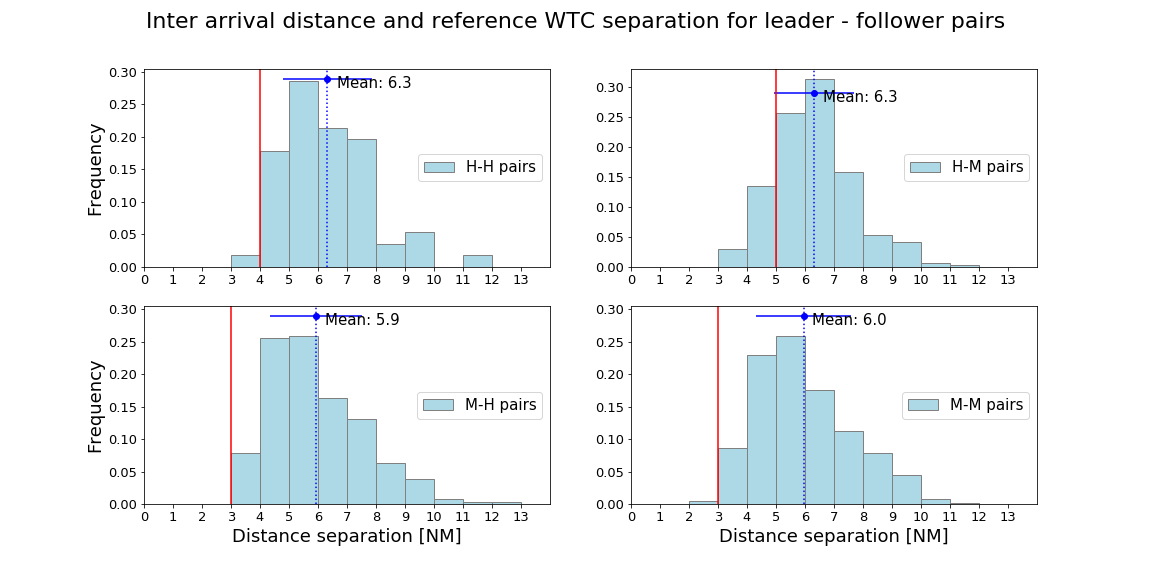
\includegraphics[width=1\textwidth]{graphics/fig_dist_separ_HH_HM_MH_MM_pairs.png}
    \caption[Distribution of distance separation for ICAO pairs]{Distribution of the WTC distance separation between selected ICAO pair categories. The red reference line indicates the separation minima for the particular pair category.}
    \label{fig:dist_separ_HH_HM_MH_MM_pairs}
\end{figure}

Another important metric derived from the data, together with the distance separation between pairs, was the landing time interval, that indicates whether AROT or the separation requirement is a limiting factor for airfield capacity. As stated in the study objective \ref{sec:study_objective} the LTI measures the time separation between aircraft calculated from the distance separation and the final approach speed. This measurement was done for each of the observed pairs and presented in Figure~\ref{fig:time_separ_HH_HM_MH_MM_pairs}, where the reference line indicates the time that a follower takes to travel the distance minima for the respective pair category. The final approach velocity for this calculation was set equal to the maximum average approach velocity from all four runways. Thus the reference time is a more liberally specified constraint. 
\begin{figure}[h]
    \centering
    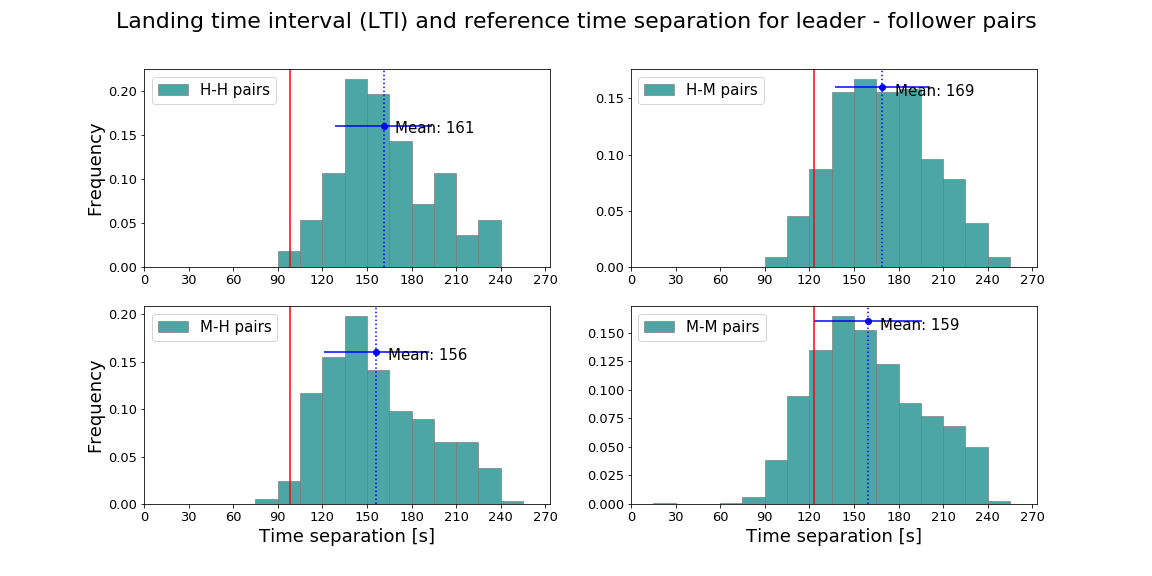
\includegraphics[width=1\textwidth]{graphics/fig_time_separ_HH_HM_MH_MM_pairs.png}
    \caption[Distribution of inter-arrival time separation for ICAO pairs]{Distribution of inter-arrival time separation for selected ICAO pair categories. The red line indicates a liberal time reference estimate for the particular pair category.}
    \label{fig:time_separ_HH_HM_MH_MM_pairs}
\end{figure}



% Please add the following required packages to your document preamble:
% \usepackage{multirow}
% \usepackage{graphicx}
\begin{table}[h]
\centering
\resizebox{\textwidth}{!}{%
\begin{tabular}{|c|c|c|c|c|c|c|c|}
\hline
\multicolumn{2}{|c|}{\multirow{2}{*}{RECAT-EU scheme}} & \multicolumn{6}{c|}{Follower}                   \\ \cline{3-8} 
\multicolumn{2}{|c|}{}                                 & CAT-A & CAT-B & CAT-C & CAT-D & CAT-E & CAT-F \\ \hline
\multirow{6}{*}{\rotatebox[origin=c]{90}{Leader}}             & CAT-A            &        & 100s  & 120s  & 140s  & 160s  & 180s  \\ \cline{2-8} 
                                    & CAT-B            &        &       &       & 100s  & 120s  & 140s  \\ \cline{2-8} 
                                    & CAT-C            &        &       &       & 80s   & 100s  & 120s  \\ \cline{2-8} 
                                    & CAT-D            &        &       &       &       &       & 120s  \\ \cline{2-8} 
                                    & CAT-E            &        &       &       &       &       & 100s  \\ \cline{2-8} 
                                    & CAT-F            &        &       &       &       &       & 80s   \\ \hline
\end{tabular}%
}
\caption[RECAT-EU time-based separation minima]{RECAT-EU WT time-based separation minima on approach and departure~\cite{rooseleer2015recat}\fxnote{This table is not referenced, maybe unnecessary, maybe move to LTI chapter!}}
\label{tab:RECAT-time}
\end{table}












%\lipsum[14-20]
%%% Local Variables: 
%%% mode: latex
%%% TeX-master: "DEGREE-NAME-YEAR"
%%% End: 
%%RUM: "Methods"
% \part{The Second Part}
\chapter{Results\label{cha:results}}

\ifdraft{In this section you discuss any issues that came up while developing
the system.  If you found something particularly interesting,
difficult, or an important learning experience, put it here.  This is
also a good place to put additional figures and data.}{}

The result section deals with presenting the different metrics discussed so far, within the RECAT-EU scheme. The data subset for the analysis was limited to four pair categories from the ICAO scheme: H-H, H-M, M-H, M-M. This simplification was done in order to filter out the insufficient data points from the other pairs for any valid conclusions.

\section{Inter-arrival Distance Separation of RECAT pairs}\label{sec:interarrival_dist_sep_RECAT}
The arrival pairs from the peak hour traffic at BIKF after re-categorisation are presented in Table~\ref{tab:pairs_mix_to_recat}. As expected from the traffic fleet analysis in \ref{ssec:traffic_mix}, most of the aircraft combined into C-C pairs. 

% Please add the following required packages to your document preamble:
% \usepackage{multirow}
% \usepackage{graphicx}
% \usepackage[table,xcdraw]{xcolor}
% If you use beamer only pass "xcolor=table" option, i.e. \documentclass[xcolor=table]{beamer}
\begin{table}[h]
\centering
\resizebox{\textwidth}{!}{%
\begin{tabular}{cc|c|c|c|c|c|c|}
\cline{3-8}
\multicolumn{1}{l}{} & \multicolumn{1}{l|}{} & \multicolumn{6}{c|}{Follower} \\ \cline{3-8} 
\multicolumn{1}{l}{} & \multicolumn{1}{l|}{} & CAT-A & CAT-B & CAT-C & CAT-D & CAT-E & CAT-F \\ \hline
\multicolumn{1}{|c|}{} & CAT-A &  &  &  & \cellcolor[HTML]{FFFFC7}1 &  &  \\ \cline{2-8} 
\multicolumn{1}{|c|}{} & CAT-B &  & \cellcolor[HTML]{FFFFC7}1 & \cellcolor[HTML]{FFFC9E}17 & \cellcolor[HTML]{FFFC9E}16 & \cellcolor[HTML]{FFFFC7}2 &  \\ \cline{2-8} 
\multicolumn{1}{|c|}{} & CAT-C &  & \cellcolor[HTML]{FFFC9E}19 & \cellcolor[HTML]{FD6864}1697 & \cellcolor[HTML]{FE996B}242 & \cellcolor[HTML]{FFCE93}41 & \cellcolor[HTML]{FFFC9E}14 \\ \cline{2-8} 
\multicolumn{1}{|c|}{} & CAT-D & \cellcolor[HTML]{FFFFC7}1 & \cellcolor[HTML]{FFFC9E}10 & \cellcolor[HTML]{FE996B}229 & \cellcolor[HTML]{FE996B}200 & \cellcolor[HTML]{FFFC9E}10 & \cellcolor[HTML]{FFFFC7}5 \\ \cline{2-8} 
\multicolumn{1}{|c|}{} & CAT-E &  & \cellcolor[HTML]{FFFFC7}1 & \cellcolor[HTML]{FFCE93}44 & \cellcolor[HTML]{FFFFC7}10 &  &  \\ \cline{2-8} 
\multicolumn{1}{|c|}{\multirow{-6}{*}{\rotatebox[origin=c]{90}{Leader}}} & CAT-F &  &  & \cellcolor[HTML]{FFFC9E}16 & \cellcolor[HTML]{FFFFC7}10 & \cellcolor[HTML]{FFFFC7}1 &  \\ \hline
\end{tabular}%
}
\caption[BIKF traffic mix sorted into RECAT-EU categories]{Number of RECAT pairs from the traffic mix at BIKF arranged into the corresponding wake categories. The majority of arrival pairs are classified as C-C.}
\label{tab:pairs_mix_to_recat}
\end{table}






\begin{figure}
    \centering
    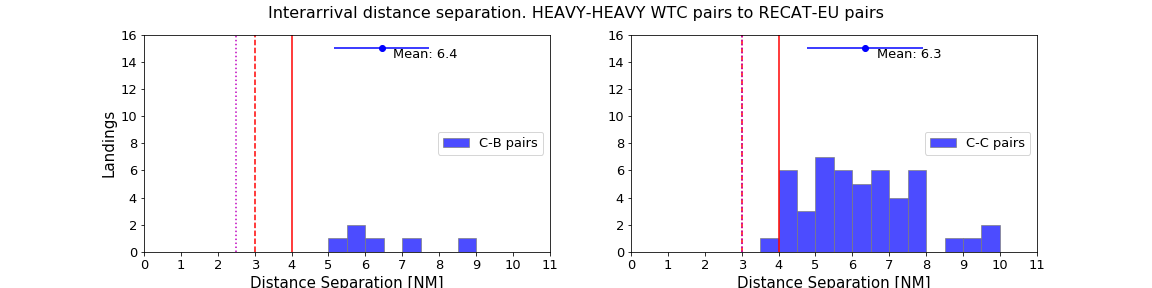
\includegraphics[width=1\textwidth]{graphics/fig_HH_to_RECAT_pairs_dist_separ.png}
    \caption[list of figures caption]{Caption}
    \label{fig:HH_to_RECAT_pairs_dist_separ}
\end{figure}

\begin{figure}
    \centering
    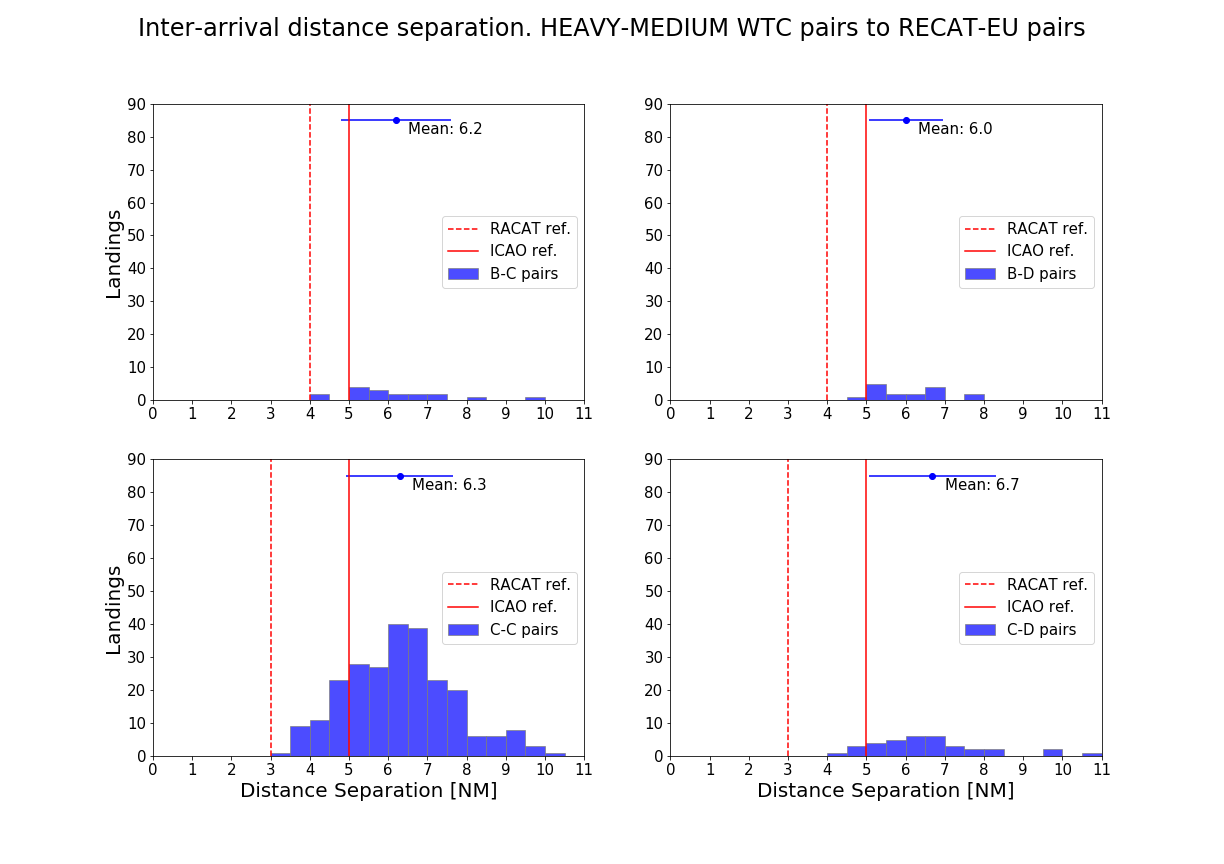
\includegraphics[width=1\textwidth]{graphics/fig_HM_to_RECAT_pairs_dist_separ.png}
    \caption[list of figures caption]{Caption}
    \label{fig:HM_to_RECAT_pairs_dist_separ}
\end{figure}

\begin{figure}
    \centering
    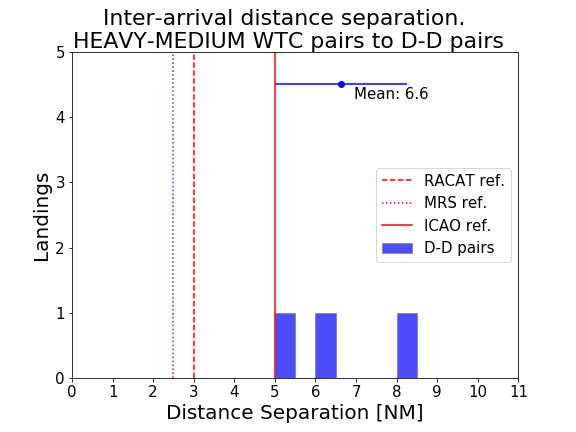
\includegraphics[width=0.5\textwidth]{graphics/fig_HM_to_DD_pairs_dist_separ.png}
    \caption[list of figures caption]{Caption}
    \label{fig:HM_to_DD_pairs_dist_separ}
\end{figure}



\begin{figure}[h]
    \centering
    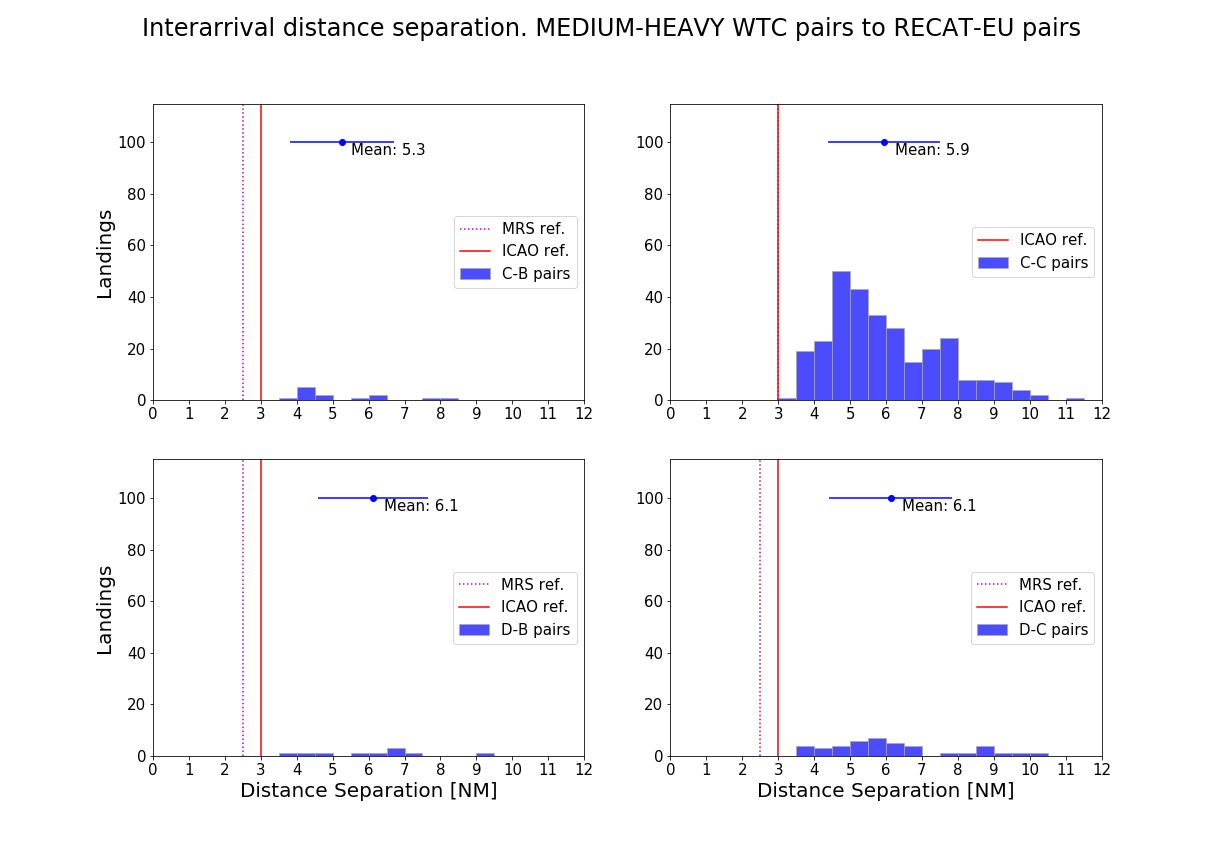
\includegraphics[width=1\textwidth]{graphics/fig_MH_to_RECAT_pairs_dist_separ.png}
    \caption[list of figures caption]{Caption}
    \label{fig:MH_to_RECAT_pairs_dist_separ}
\end{figure}

\begin{figure}[h]
    \centering
    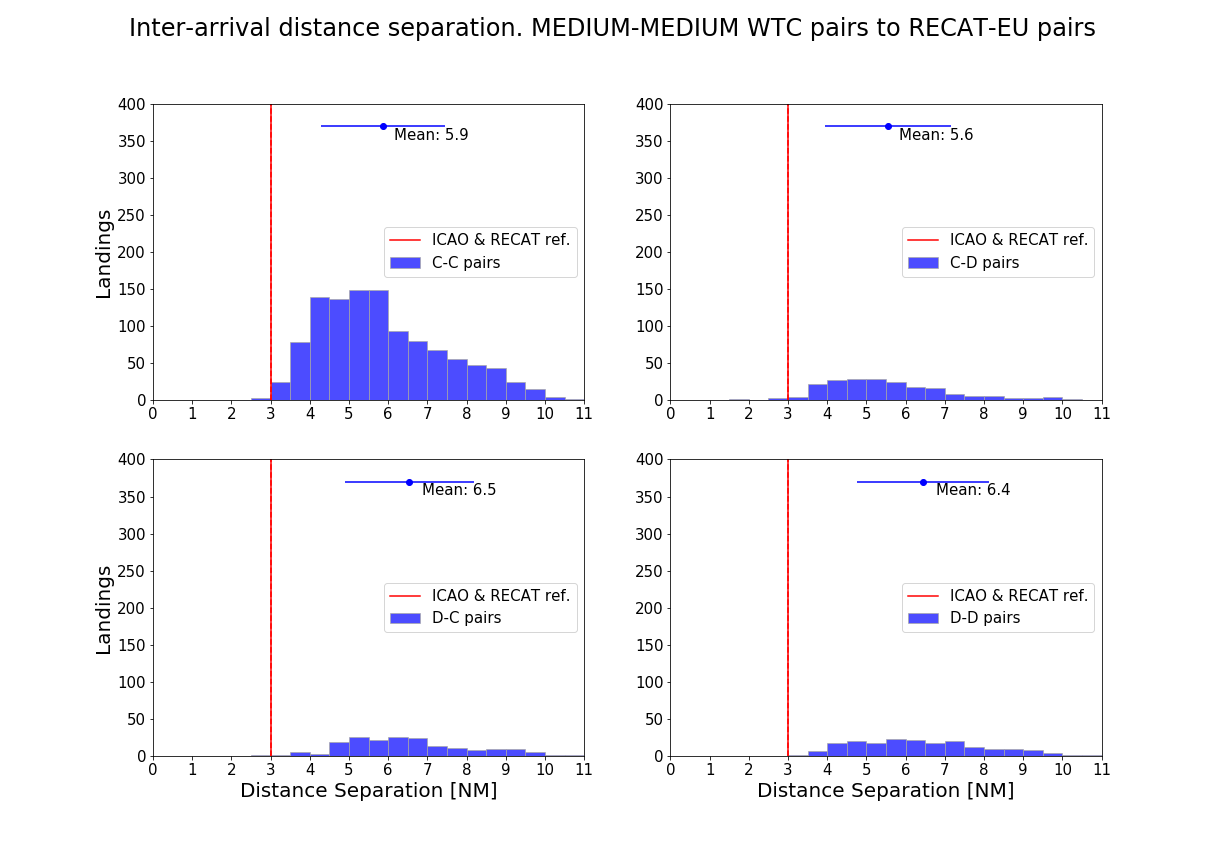
\includegraphics[width=1.0\textwidth]{graphics/fig_MM_to_RECAT_pairs_dist_separ.png}
    \caption[list of figures caption]{Caption}
    \label{fig:MM_to_RECAT_pairs_dist_separ}
\end{figure}

\begin{figure}[h]
    \centering
    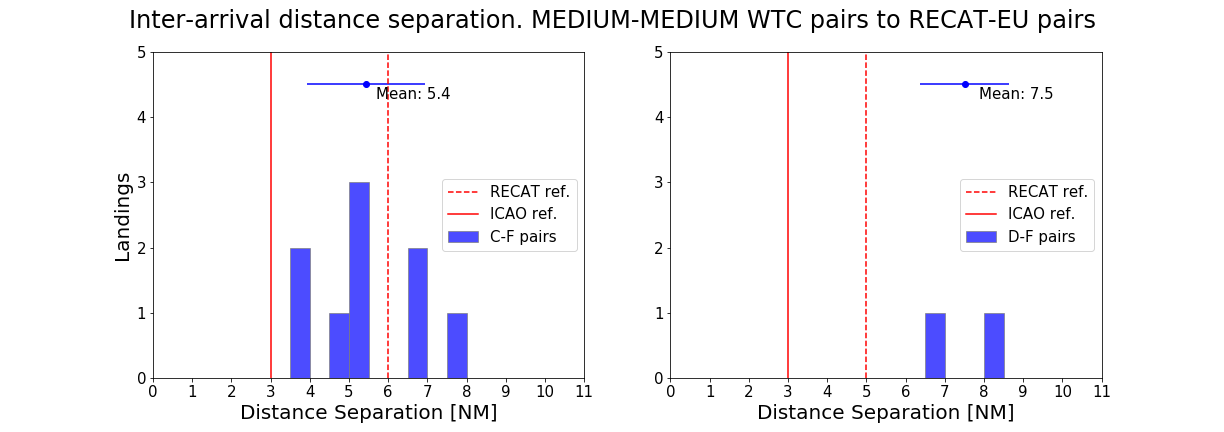
\includegraphics[width=1\textwidth]{graphics/fig_MM_to_CF_and_DF_pairs_dist_separ.png}
    \caption[list of figures caption]{Caption}
    \label{fig:MM_to_CF_and_DF_pairs_dist_separ}
\end{figure}


\section{Runway Occupancy and Landing Time Interval for RECAT pairs}




\begin{figure}[h]
    \centering
    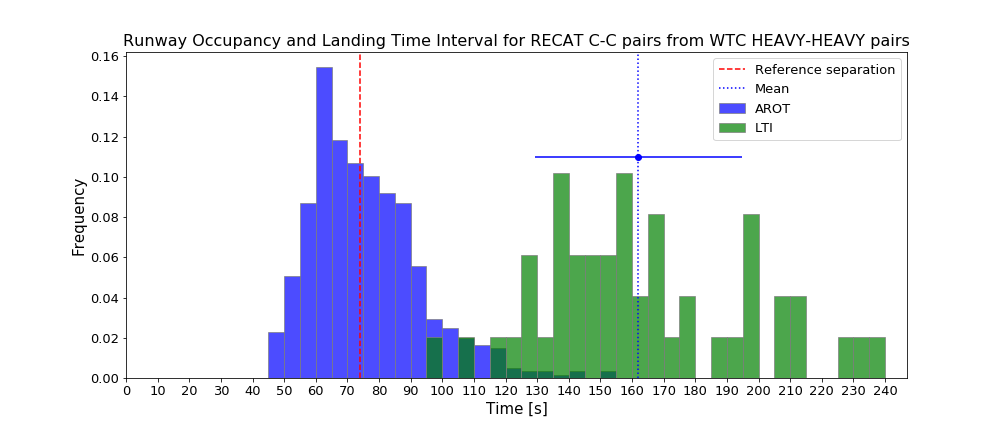
\includegraphics[width=1\textwidth]{graphics/fig_CC_from_HH_pairs_time_sep.png}
    \caption[list of figures caption]{Caption}
    \label{fig:CC_from_HH_pairs_time_sep}
\end{figure}




\begin{figure}[h]
    \centering
    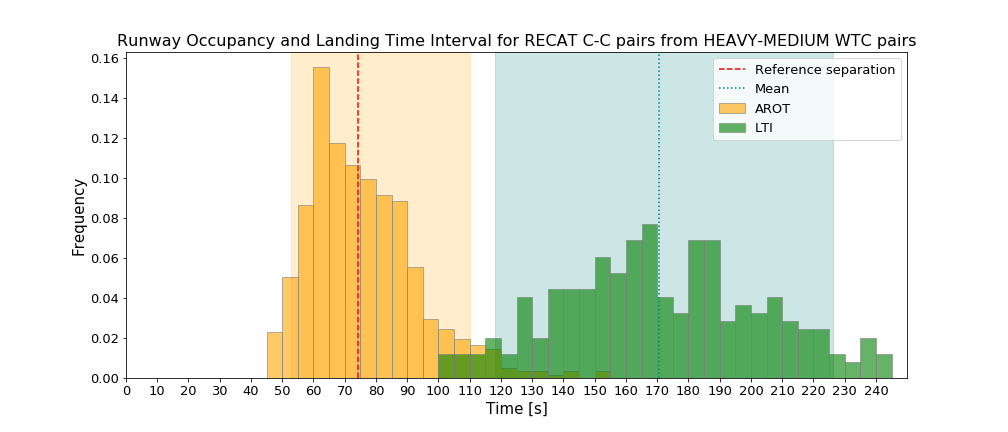
\includegraphics[width=1\textwidth]{graphics/fig_CC_from_HM_pairs_time_sep.png}
    \caption[list of figures caption]{Caption}
    \label{fig:CC_from_HM_pairs_time_sep}
\end{figure}

\begin{figure}[h]
    \centering
    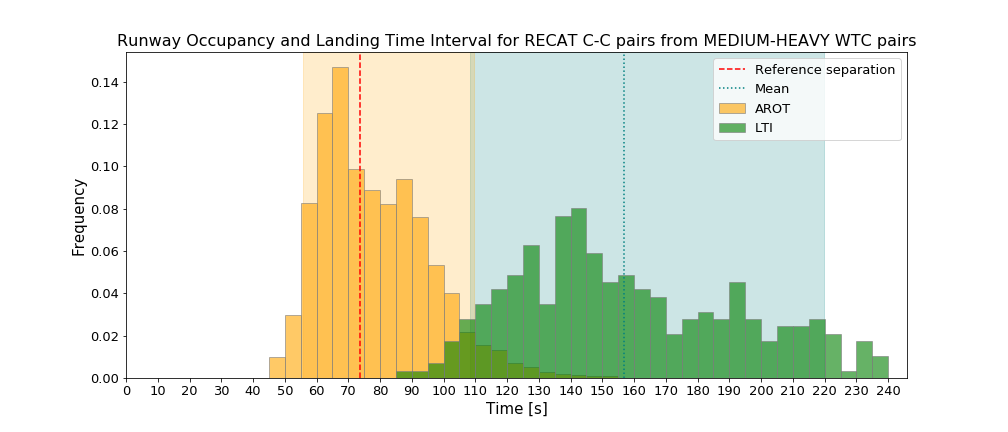
\includegraphics[width=1\textwidth]{graphics/fig_CC_from_MH_pairs_time_sep.png}
    \caption[list of figures caption]{Caption}
    \label{fig:CC_from_MH_pairs_time_sep}
\end{figure}

\begin{figure}[h]
    \centering
    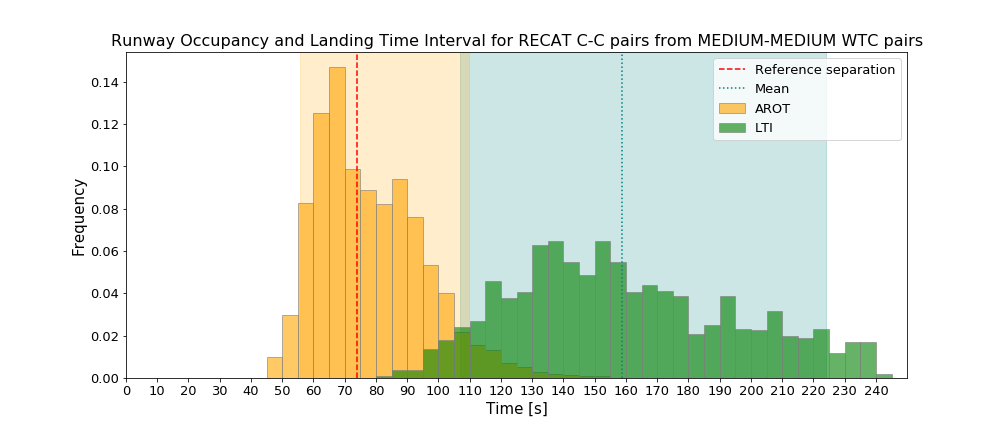
\includegraphics[width=1\textwidth]{graphics/fig_CC_from_MM_pairs_time_sep.png}
    \caption[list of figures caption]{Caption}
    \label{fig:CC_from_MM_pairs_time_sep}
\end{figure}

\begin{figure}[h]
    \centering
    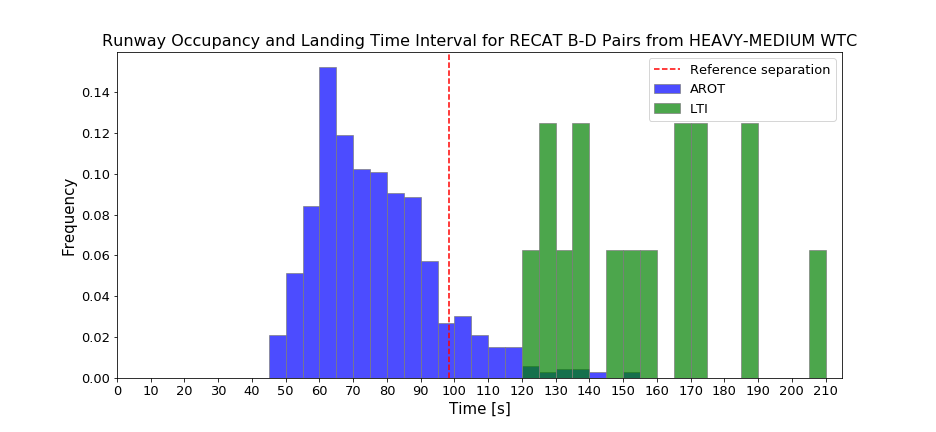
\includegraphics[width=1\textwidth]{graphics/fig_BD_from_HM_pairs_time_sep.png}
    \caption[list of figures caption]{Caption}
    \label{fig:BD_from_HM_pairs_time_sep}
\end{figure}







% \lipsum[28-34]

%%% Local Variables: 
%%% mode: latex
%%% TeX-master: "DEGREE-NAME-YEAR"
%%% End: 
%%RUM: "Results"



\chapter{Summary-WORK IN PROGRESS}\label{cha:summary}

Airfield capacity is influenced by two major factors: runway occupancy and wake turbulence separation. Already, the analysis of those metrics has been performed by Isavia within the current ICAO wake turbulence scheme. Wake turbulence categories in use at BIKF and the arrival runway occupancy times show that in most of the cases the AROT is a limiting factor for increase of the airfield throughput.  

Different variables affect the AROT, such as the existence and usage of rapid-exit taxiways, weather conditions and the traffic mix. Two rapid-exit taxiways became operational in 2017 (taxiway TWY~A-1 and TWY~B-1). The usage of TWY~B-1 on runway RWY~28 has managed to decrease the AROT by more than 33\% (37 seconds) on average during the winter and 31\% (31 seconds) during the summer months. The seasonal variations of the AROT were also examined and showed a difference of almost 10\% on average. The weather conditions determine runway surface conditions that affect braking action, the strength and direction of winds and visibility. 

The traffic fleet at BIKF was primarily from the CAT-C and CAT-D wake categories that combined represent 96\% of the arrivals and were so far the aircraft with the smallest AROT on average. Nevertheless the above conditions were insufficient to produce AROT~$\leq~50$ seconds, which is one requirement for reducing the radar separation minima (MRS) for aircraft on final approach to the 2,5 NM minimum. The average arrival runway occupancy time for BIKF was 78 seconds. 

The runway occupancy in turn has effect on the landing time intervals, which is also governed by the wake turbulence requirements.
The analysis of the re-categorisation requirements for BIKF show that for certain pairs the wake turbulence separation could be reduced by~1--2~NM, while for a few others the separation would increase by~2--3~NM. Reduced wake turbulence separation will affect most of the Heavy-Heavy and the Heavy-Medium pairs. Separation will increase for Medium-Medium pairs that are re-categorised as C-F and D-F pairs, but the number of those cases for Keflavík Airport is relatively small.



\chapter{Conclusion-WORK IN PROGRESS\label{cha:conclusions}}

This study uses measured data from the ADS-B surveillance system at Keflavík International Airport~(BIKF) to estimate the arrival runway occupancy time~(AROT) and the wake turbulence separation and aims to validate the constraints of implementing the RECAT-EU wake  separation scheme for BIKF. The focus is on arrival aircraft pairs during peak hours and the observed time period is fourteen months (from 4 October 2017 to 30 November 2018). 

The majority of the fleet mix though will experience no change of wake turbulence separation with the implementation of the RECAT-EU scheme. The separation requirement for the most of the ICAO Medium-Medium pairs remains 3~NM after re-categorisation and the same is true for Medium-Heavy pairs. The combined share of the aircraft that will experience no change to required wake turbulence separation is 83,5\%. 

The wake distance separation was transferred into time separation and defined as the landing time interval~(LTI), in order to compare it to arrival runway occupancy time.
The correlation of arrival runway occupancy and landing time intervals for the predominant C-C pairs revealed that even though a decrease of the LTI is apparently possible, the AROT is a limiting factor for increased runway throughput. Not only do the landing frequency distributions of the two metrics overlap to some extent but also the reference time line is well within the AROT range. One way the conflict between the AROT and LTI can manifest itself is through a missed approach due to the incorrect presence of another aircraft on the runway designated for landing.

% \chapter{Conclusion-WORK IN PROGRESS\label{cha:conclusions}}
The analysis of landing aircraft at Keflavík International, when the airport operates at high loads, shows that rapid-exits on runways have a strong influence of arrival runway occupancy times. Optimised position of rapid-exits in context with the traffic fleet can reduce AROT by 1/3.% The reduction can be greater still if the weather conditions are favourable, even though its effect of is intermittent and not decisive for AROT.

Under the RECAT-EU scheme, the wake turbulence separation will remain unchanged for the majority of the aircraft pairs arriving at BIKF during peak hours. A predominant part of the traffic mix (69,9\%) is currently classified as Medium-Medium within the ICAO wake turbulence categories and after re-categorisation the reference separation between most of those aircraft pairs (98\%) remains 3 NM. One observation from the frequency distribution of the landing time intervals is the wide range over which the times are spread. If the frequency distribution is compressed, this will create opportunity for overall decrease of the inter-arrival time intervals by shifting the distribution closer to the required minimum separation. This possibility can potentially accommodate more landings per time interval and raise runway capacity.

Arrival runway occupancy times and wake turbulence separation requirements interact to formulate the capacity of an airfield. In the case with Keflavík Airport, high arrival runway occupancy times are an obstacle for increased runway capacity, despite the prospect of decreased wake turbulence separation within the RECAT-EU scheme. The observed arrival runway occupancy time is a limiting factor for increase of the runway throughput for the selected aircraft pairs from the current fleet mix at Keflavík Airport.

Although the study examines the constraints of the airfield in connection with RECAT, it only considers the data for arriving aircraft. The analysis becomes more complex and involved when arrival-departure sequencing is considered. Estimating the constraints on airfield capacity for each of the runways with regard to arrivals and departures is a subject for future work. Creating a simulation of the arrival-departure sequencing and assessing the effect of wind and weather conditions on runway occupancy times can also be considered a continuation of this work.

% \lipsum[35-41]


% \lipsum[42-43]
% \lipsum[44-50]
%%% Local Variables: 
%%% mode: latex
%%% TeX-master: "DEGREE-NAME-YEAR"
%%% End: 
%%RUM: "Discussion"

%% ---------------------------------------------------------------
\printbibliography{} %%RUM: "References"

%% If appendices are needed, uncomment the following line
%% and include the appendices in separate files
\appendix{}%%RUM: "Appendicies (as appropriate)



\chapter{Runway Usage}\label{app:RWY_usage}


\begin{figure}[h]
    \centering
    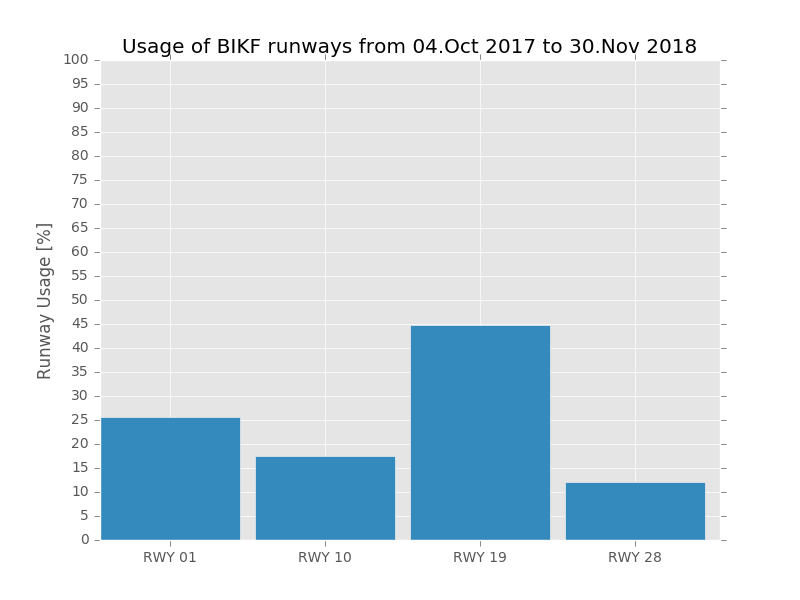
\includegraphics[width=0.8\textwidth]{graphics/fig_runway_usage_2017-10-04_to_2018-11-30.png}
    \caption[Runway usage at BIKF]{Overall runway usage at BIKF for a period of one year since October 2017. Almost half of all arrivals during that period (44,7\%) use RWY-19, followed by RWY-01 (25,7\%) and RWY-10 (17.6\%). The summer traffic favoured RWY-19 with 52.8\%~(Figure~\ref{fig:runway_usage_summer}), while during the winter season some of those arrivals were diverted towards RWY-01 and RWY-10~(Figure~\ref{fig:runway_usage_summer}). RWY-28 was least used despite its rapid-exit TWY B-1.}
    \label{fig:runway_usage}
\end{figure}

\begin{figure}[h]
    \centering
    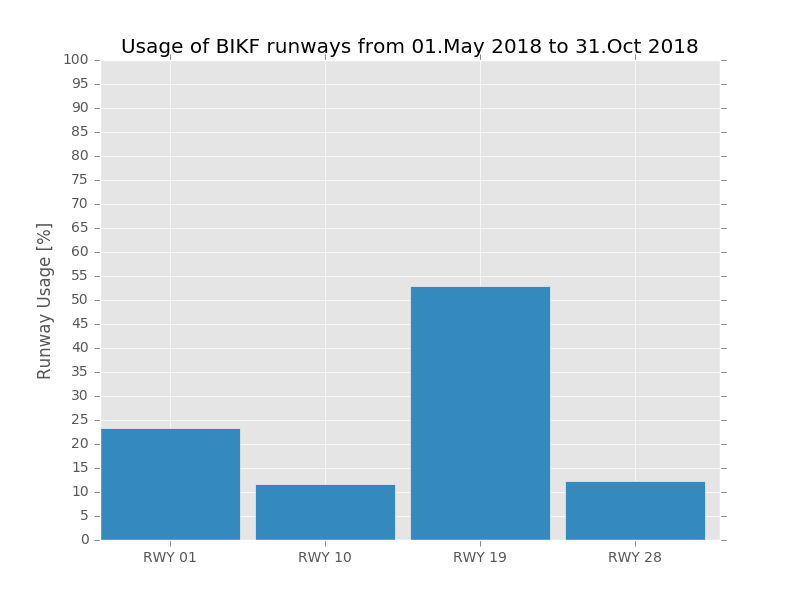
\includegraphics[width=0.7\textwidth]{graphics/fig_runway_usage_summer}
    \caption[Summer runway usage at BIKF]{The summer traffic favours RWY-19 (52,8\%), followed by RWY-01 (23,3\%), while RWY-10 and RWY-28 are with 11,6\% and 12,3\% respectively.}
    \label{fig:runway_usage_summer}
\end{figure}

\begin{figure}[h]
    \centering
    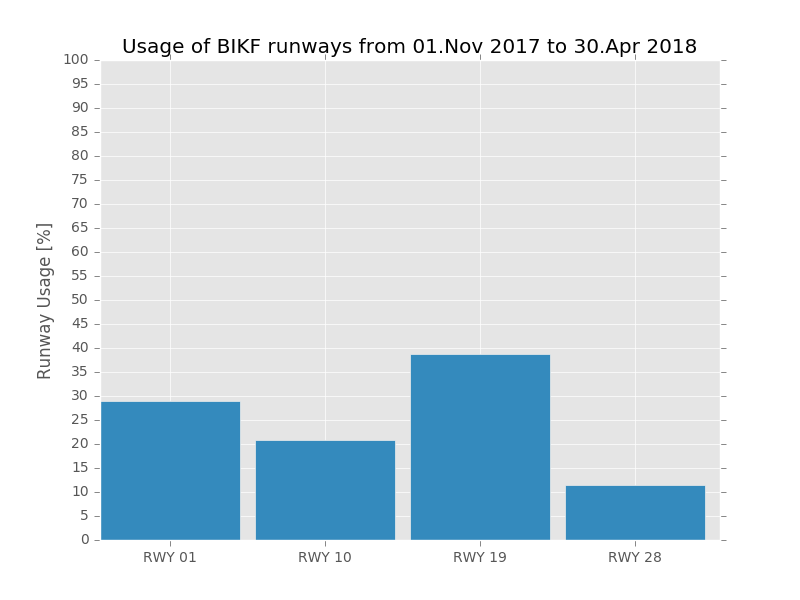
\includegraphics[width=0.7\textwidth]{graphics/fig_runway_usage_winter}
    \caption[Winter runway usage at BIKF]{The winter traffic at BIKF is slightly more evenly distributed among runways but still favours RWY-19 (38,8\%),followed by RWY-01 with 28,9\%, RWY-10 (20,8\%) and RWY-28 (11,4\%).}
    \label{fig:runway_usage_winter}
\end{figure}

\clearpage
\chapter{Arrival Runway Occupancy Times\label{app:AROTs}}



% Please add the following required packages to your document preamble:
% \usepackage{graphicx}
\begin{table}[h]
\centering
\resizebox{0.8\textwidth}{!} & \multicolumn{1}{l|}{50\%} & \multicolumn{1}{l|}{75\%} & \multicolumn{1}{l|}{max} \\ \hline
\multicolumn{1}{|l|}{Summer} & \multicolumn{1}{r|}{764} & 85 & 20 & 46 & 70 & 86 & 99 & 153 \\ \hline
\multicolumn{1}{|l|}{Winter} & \multicolumn{1}{r|}{263} & 100 & 17 & 55 & 87 & 98 & 111 & 156 \\ \hline
\end{tabular}%
}
\caption[AROTs RWY-01 pre rapid-exit by season]{AROTs for runway RWY-01 pre-rapid-exit TWY A-1 by season}
\label{tab:season_AROT_stats_RWY01_pre_fast_exit}
\end{table}

% Please add the following required packages to your document preamble:
% \usepackage{graphicx}
\begin{table}[h]
\centering
\resizebox{0.8\textwidth}{!} & \multicolumn{1}{l|}{50\%} & \multicolumn{1}{l|}{75\%} & \multicolumn{1}{l|}{max} \\ \hline
\multicolumn{1}{|l|}{Summer} & \multicolumn{1}{r|}{1879} & 84 & 22 & 46 & 64 & 86 & 98 & 152 \\ \hline
\multicolumn{1}{|l|}{Winter} & \multicolumn{1}{r|}{290} & 88 & 26 & 47 & 63 & 90 & 106 & 153 \\ \hline
\end{tabular}%
}
\caption[AROTs RWY-01 post rapid-exit by season]{AROTs for runway RWY-01 post-rapid-exit TWY A-1 by season}
\label{tab:season_AROT_stats_RWY01_post_fast_exit}
\end{table}

% Please add the following required packages to your document preamble:
% \usepackage{graphicx}
\begin{table}[h]
\centering
\resizebox{0.8\textwidth}{!} & \multicolumn{1}{l|}{50\%} & \multicolumn{1}{l|}{75\%} & \multicolumn{1}{l|}{max} \\ \hline
\multicolumn{1}{|l|}{Summer} & \multicolumn{1}{r|}{553} & 99 & 12 & 46 & 91 & 98 & 106 & 153 \\ \hline
\multicolumn{1}{|l|}{Winter} & \multicolumn{1}{r|}{249} & 110 & 13 & 60 & 100 & 108 & 117 & 155 \\ \hline
\end{tabular}%
}
\caption[AROTs RWY-28 pre rapid-exit by season]{AROTs for runway RWY-28 pre-rapid-exit TWY B-1 by season}
\label{tab:season_AROT_stats_RWY28_pre_fast_exit}
\end{table}

% Please add the following required packages to your document preamble:
% \usepackage{graphicx}
\begin{table}[h]
\centering
\resizebox{0.8\textwidth}{!} & \multicolumn{1}{l|}{50\%} & \multicolumn{1}{l|}{75\%} & \multicolumn{1}{l|}{max} \\ \hline
\multicolumn{1}{|l|}{Summer} & 401 & 68 & 14 & 49 & 60 & 66 & 72 & 155 \\ \hline
\multicolumn{1}{|l|}{Winter} & 69 & 73 & 13 & 49 & 63 & 72 & 79 & 105 \\ \hline
\end{tabular}%
}
\caption[AROTs RWY-28 post rapid-exit by season]{AROTs for runway RWY-28 post-rapid-exit TWY B-1 by season}
\label{tab:season_AROT_stats_RWY28_post_fast_exit}
\end{table}

% Please add the following required packages to your document preamble:
% \usepackage{graphicx}
\begin{table}[h]
\centering
\resizebox{0.8\textwidth}{!} & \multicolumn{1}{l|}{50\%} & \multicolumn{1}{l|}{75\%} & \multicolumn{1}{l|}{max} \\ \hline
\multicolumn{1}{|l|}{RWY 01} & 963 & 85 & 21 & 46 & 68 & 88 & 100 & 152 \\ \hline
\multicolumn{1}{|l|}{RWY 10} & 852 & 85 & 11 & 61 & 78 & 84 & 91 & 155 \\ \hline
\multicolumn{1}{|l|}{RWY 19} & 1511 & 67 & 10 & 46 & 61 & 66 & 71 & 155 \\ \hline
\multicolumn{1}{|l|}{RWY 28} & 401 & 68 & 14 & 49 & 60 & 66 & 72 & 155 \\ \hline
\end{tabular}%
}
\caption[AROTs for the air traffic mix by runway for the summer]{AROT statistics for the air traffic mix at KEF by runway for the summer of 2018. The count is the number of landings during peak hours.}
\label{my-label3}
\end{table}

% Please add the following required packages to your document preamble:
% \usepackage{graphicx}
\begin{table}[h]
\centering
\resizebox{0.8\textwidth}{!} & \multicolumn{1}{l|}{50\%} & \multicolumn{1}{l|}{75\%} & \multicolumn{1}{l|}{max} \\ \hline
\multicolumn{1}{|l|}{RWY 01} & 290 & 88 & 26 & 47 & 63 & 90 & 106 & 153 \\ \hline
\multicolumn{1}{|l|}{RWY 10} & 338 & 93 & 12 & 70 & 85 & 91 & 100 & 144 \\ \hline
\multicolumn{1}{|l|}{RWY 19} & 259 & 72 & 13 & 51 & 65 & 69 & 75 & 140 \\ \hline
\multicolumn{1}{|l|}{RWY 28} & 69 & 73 & 13 & 49 & 63 & 72 & 79 & 105 \\ \hline
\end{tabular}%
}
\caption[AROTs for the air traffic mix by runway for the winter]{AROT statistics for the air traffic mix at KEF by runway for the winter season. The count is the number of landings during peak hours since October 2017}
\label{my-label4}
\end{table}

% Please add the following required packages to your document preamble:
% \usepackage{graphicx}
% \usepackage[table,xcdraw]{xcolor}
% If you use beamer only pass "xcolor=table" option, i.e. \documentclass[xcolor=table]{beamer}
\begin{table}[h]
\centering
\resizebox{0.8\textwidth}{!} & \multicolumn{1}{l|}{50\%} & \multicolumn{1}{l|}{75\%} & \multicolumn{1}{l|}{max} \\ \hline
\rowcolor[HTML]{DAE8FC} 
\multicolumn{1}{|l|}{\cellcolor[HTML]{DAE8FC}January} & 95 & 86 & 20 & 54 & 70 & 85 & 96 & 136 \\ \hline
\rowcolor[HTML]{DAE8FC} 
\multicolumn{1}{|l|}{\cellcolor[HTML]{DAE8FC}February} & 80 & 87 & 16 & 52 & 75 & 86 & 93 & 144 \\ \hline
\rowcolor[HTML]{DAE8FC} 
\multicolumn{1}{|l|}{\cellcolor[HTML]{DAE8FC}March} & 215 & 84 & 18 & 47 & 70 & 85 & 95 & 150 \\ \hline
\rowcolor[HTML]{DAE8FC} 
\multicolumn{1}{|l|}{\cellcolor[HTML]{DAE8FC}April} & 221 & 82 & 17 & 47 & 69 & 81 & 93 & 139 \\ \hline
\rowcolor[HTML]{FFFC9E} 
\multicolumn{1}{|l|}{\cellcolor[HTML]{FFFC9E}May} & 386 & 75 & 13 & 46 & 67 & 74 & 83 & 140 \\ \hline
\rowcolor[HTML]{FFFC9E} 
\multicolumn{1}{|l|}{\cellcolor[HTML]{FFFC9E}June} & 647 & 73 & 16 & 47 & 62 & 68 & 80 & 155 \\ \hline
\rowcolor[HTML]{FFFC9E} 
\multicolumn{1}{|l|}{\cellcolor[HTML]{FFFC9E}July} & 729 & 72 & 16 & 46 & 61 & 68 & 77 & 155 \\ \hline
\rowcolor[HTML]{FFFC9E} 
\multicolumn{1}{|l|}{\cellcolor[HTML]{FFFC9E}August} & 724 & 80 & 18 & 46 & 64 & 81 & 91 & 148 \\ \hline
\rowcolor[HTML]{FFFC9E} 
\multicolumn{1}{|l|}{\cellcolor[HTML]{FFFC9E}September} & 632 & 78 & 18 & 46 & 64 & 75 & 88 & 152 \\ \hline
\rowcolor[HTML]{FFFC9E} 
\multicolumn{1}{|l|}{\cellcolor[HTML]{FFFC9E}October} & 609 & 79 & 17 & 46 & 66 & 76 & 91 & 155 \\ \hline
\rowcolor[HTML]{DAE8FC} 
\multicolumn{1}{|l|}{\cellcolor[HTML]{DAE8FC}November} & 239 & 84 & 23 & 48 & 66 & 82 & 99 & 151 \\ \hline
\rowcolor[HTML]{DAE8FC} 
\multicolumn{1}{|l|}{\cellcolor[HTML]{DAE8FC}December} & 106 & 87 & 23 & 51 & 69 & 86 & 99 & 153 \\ \hline
\end{tabular}%
}
\caption[AROTs for the air traffic mix by month]{AROT statistics for the air traffic mix at BIKF by month. The count is the number of landings during peak hours from October 2017 til November 2018. The colour fields indicate a subjective separation of the data into summer and winter season, based on mean AROT value. Months with mean AROT $\leq$ 80 seconds were classified as summer, and the remaining as winter.}
\label{tab:month2season_arot}
\end{table}

\clearpage
\chapter{Inter-arrival time and distance separation}\label{app:time_and_dist_sep}

\begin{figure}[h]
    \centering
    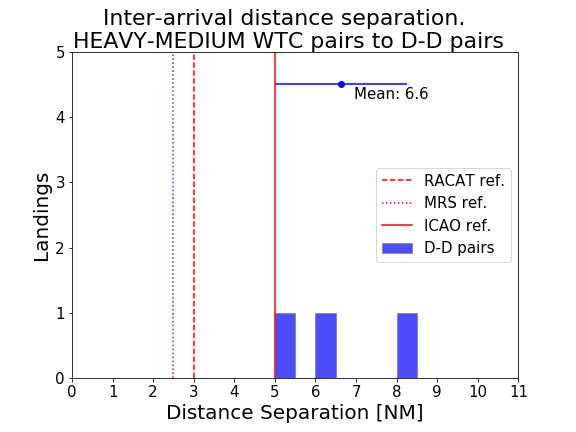
\includegraphics[width=0.5\textwidth]{graphics/fig_HM_to_DD_pairs_dist_separ.png}
    \caption[Inter-arrival distance separation of H-M pairs to D-D pairs into the RECAT-EU scheme]{Inter-arrival distance separation after re-categorisation of H-H pairs to D-D pairs into the RECAT-EU scheme.}
    \label{fig:HM_to_DD_pairs_dist_separ}
\end{figure}


% Please add the following required packages to your document preamble:
% \usepackage{multirow}
% \usepackage{graphicx}
\begin{table}[h]
\centering
\resizebox{0.8\textwidth}{!}{%
\begin{tabular}{|c|c|c|c|c|c|c|c|}
\hline
\multicolumn{2}{|c|}{\multirow{2}{*}{RECAT-EU scheme}} & \multicolumn{6}{c|}{Follower}                   \\ \cline{3-8} 
\multicolumn{2}{|c|}{}& CAT-A & CAT-B & CAT-C & CAT-D & CAT-E & CAT-F \\ \hline
\multirow{6}{*}{\rotatebox[origin=c]{90}{Leader}}& CAT-A&& 100s  & 120s  & 140s  & 160s  & 180s  \\ \cline{2-8}
& CAT-B&&&& 100s  & 120s  & 140s  \\ \cline{2-8} 
& CAT-C&&&& 80s   & 100s  & 120s  \\ \cline{2-8} 
& CAT-D&&&&&& 120s  \\ \cline{2-8} 
& CAT-E&&&&&& 100s  \\ \cline{2-8} 
& CAT-F&&&&&& 80s   \\ \hline
\end{tabular}%
}
\caption[RECAT-EU time-based separation minima]{RECAT-EU WT time-based separation minima on approach and departure~\cite{rooseleer2015recat}}
\label{tab:RECAT-time}
\end{table}



\begin{figure}[h]
    \centering
    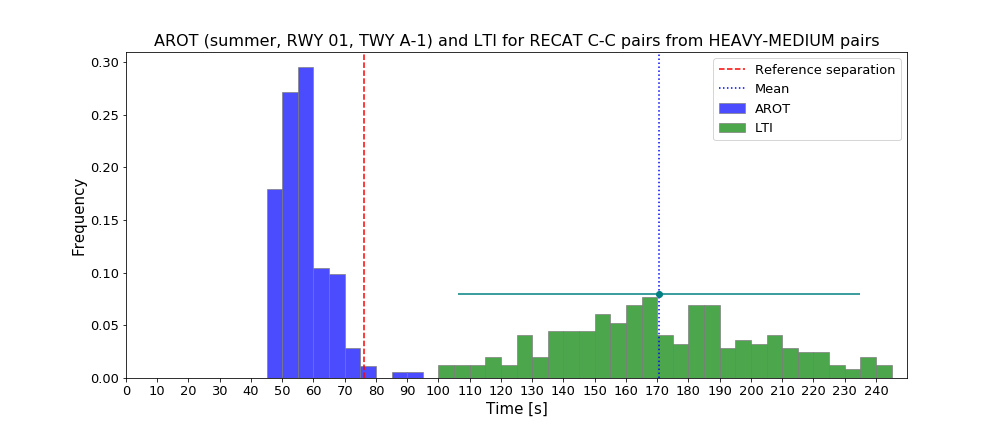
\includegraphics[width=1.0\textwidth]{graphics/fig_best_CC_from_HM_pairs_time_sep.png}
    \caption[AROT and LTI of C-C pairs from ICAO H-M pairs on RWY~19]{AROT and landing time intervals of C-C pairs originating from ICAO H-M pairs for RWY-19 during the summer season. The dashed red line indicates the RECAT-EU reference time separation for the C-C pairs.}
    \label{fig:best_CC_from_HM_pairs_time_sep}
\end{figure}


\clearpage
\chapter{ADS-B Standard Data Items}\label{app:adsb_items}

\begin{figure}[h]
    \centering
    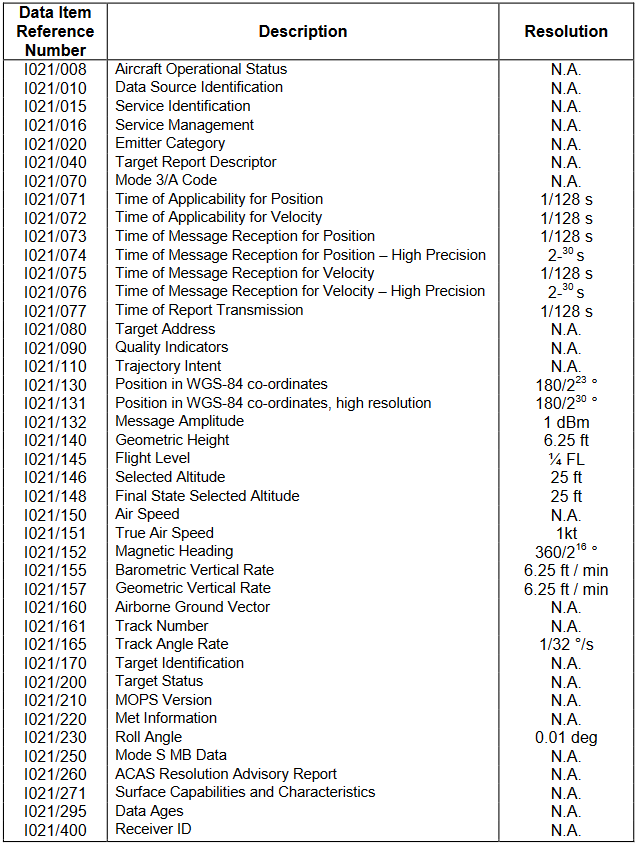
\includegraphics[width=0.7\textwidth]{graphics/ads_b_items.png}
    \caption[ADS-B Standard Data Items]{ADS-B Standard Data Items \cite[p. 8]{ASTERIX_ADS-B_specs}.}
    \label{fig:adsb_items}
\end{figure}


\clearpage
\chapter{BIKF Wind Rose}\label{app:wind_rose}

\begin{figure}[h]
    \centering
    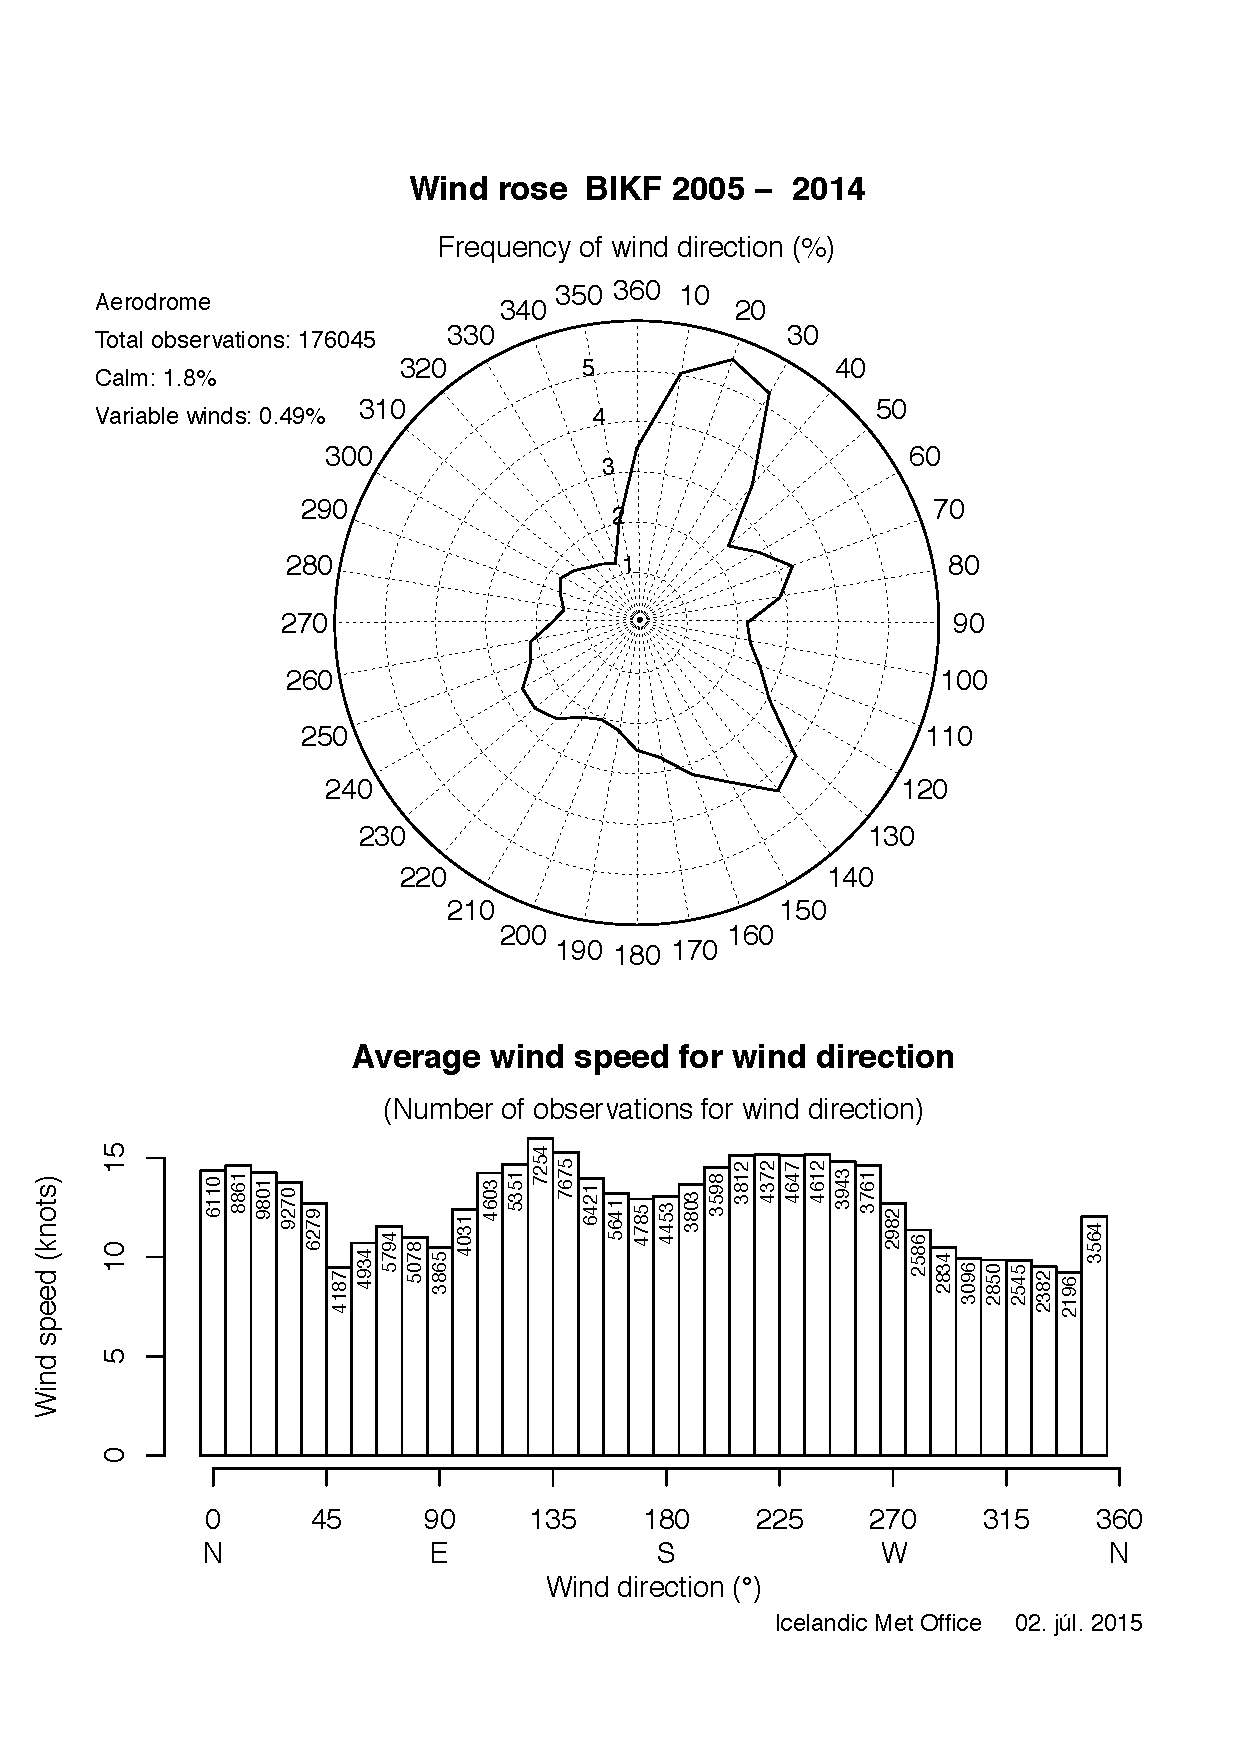
\includegraphics[width=0.7\textwidth]{graphics/BIKF_windrose_2005-2014.pdf}
    \caption[BIKF Wind Rose]{Wind rose - frequency, direction and strength of winds at BIKF aerodrome \cite{wind_rose_2014}.}
    \label{fig:BIKF_wind_rose}
\end{figure}
% ----------------------------


% \chapter{Code}\label{cha:code}
% You can put code in your document using the listings package, which is
% loaded by default in \path{custom.tex}.  Be aware that the listings
% package does not put code in your document if you are in draft mode
% unless you set the \texttt{forcegraphics} option.

% There is an example java (Listing~\ref{src:Data_Bus.java}) and XML
% file (Listing~\ref{src:AndroidManifest.xml}).  Thanks to the
% \texttt{url} package, you can typeset OSX and unix paths like this:
% \path{/afs/rnd.ru.is/project/thesis-template}.  Windows paths:
% \path{C:\windows\temp\ }.  You can also typeset them using the menukey
% package, but it tends to delete the last separator and has other
% complications.\footnote{The menukey package has issues with biblatex,
%   read \path{custom.tex} for more information.}

% If you are trying to include multiple different languages, you should
% go read the documentation and set these up in \path{custom.tex}.  You
% will save yourself a lot of effort, especially if you have to fix
% anything.

% %I have put the source code in the \directory{src/} folder.
% \lstinputlisting[language=Java, firstline=1,
% lastline=40, caption={Data\_Bus.java: Setting up the class.},
% label={src:Data_Bus.java}]{src/Data_Bus.java}

% \lstinputlisting[language={[android]XML}, firstline=1, lastline=20,
% caption={AndroidManifest.xml: Configuration for the Android UI.},
% label={src:AndroidManifest.xml}]{src/AndroidManifest.xml}

%%% Local Variables: 
%%% mode: latex
%%% TeX-master: "DEGREE-NAME-YEAR"
%%% End: 
 % as an example, perhaps some of your code
% \input{app2}
%\backmatter{} % Sections after this don't get numbers
%% We prefer that all elements be numbered

%%%%%%%%%%%%% SHOW INDEX %%%%%%%%%%%%%%%%%%
%% Index, optional.  A good idea on longer documents

% You can put instructions at the beginning of the index:
%\renewcommand{\preindexhook}{%
%  The first page number is usually, but not always,
%  the primary reference to the indexed topic.\vskip\onelineskip}

%% You may have to run "makeindex <FILENAME>" to have it be generated
%% Depending upon which package you chose.
%% 
\clearforchapter{}
\printindex{}%%RUM: Not mentioned

%\backcover{}%%RUM: "Back cover (only Phd)
\end{document}

%% ---------------------------------------------------------------

%%% Local Variables:
%%% mode: latex
%%% TeX-master: t
%%% TeX-engine: xetex
%%% End:
